\documentclass{article}
% \usepackage[UTF8]{ctex}

\usepackage[colorlinks]{hyperref}
\usepackage[fontsize=9.5pt]{fontsize}
\usepackage{geometry}
\usepackage{multicol}
\usepackage{url}
\usepackage{booktabs}
\usepackage[most]{tcolorbox}
\usepackage{xcolor}
\usepackage{amsmath, amsfonts, amssymb, amsthm}
\usepackage{ulem}
\usepackage{enumitem}
\usepackage{titlesec}
\titleformat{\section}
  {\normalfont\sffamily\Large\bfseries}
  {\thesection}{1em}{}
\titleformat{\subsection}
  {\normalfont\sffamily\large\bfseries}
  {\thesubsection}{1em}{}
  
\geometry{a4paper, left=1.5cm, right=1.5cm, top=2cm, bottom=2.5cm}
\setlength\columnsep{15pt} 
\setlength\parindent{0em}

% \renewcommand{\familydefault}{\sfdefault}
% \CTEXsetup[format={\centering}]{section}
% \CTEXsetup[nameformat={\zihao{4}\heiti}]{section}
% \CTEXsetup[titleformat={\zihao{4}\heiti}]{section}
% \CTEXsetup[format={}]{subsection}
% \CTEXsetup[nameformat={\zihao{-4}\heiti}]{subsection}
% \CTEXsetup[titleformat={\zihao{-4}\heiti}]{subsection}
% % \setCJKmainfont{SimSun}[BoldFont=HeiTi,ItalicFont=KaiTi]
% % \setCJKmainfont{SimSun}
% \renewcommand{\textbf}[1]{{\heiti #1}}
\setlist[itemize]{leftmargin=*}

\definecolor{tssteelblue}{RGB}{70,130,180}
\definecolor{tsorange}{RGB}{255,138,88}
\definecolor{tsblue}{RGB}{23,74,157}
\definecolor{tsforestgreen}{RGB}{21,122,81}
\definecolor{tsyellow}{RGB}{255,185,88}
\definecolor{tsgrey}{RGB}{200,200,200}

\definecolor{codegreen}{rgb}{0,0.6,0}
\definecolor{codegray}{rgb}{0.5,0.5,0.5}
\definecolor{codepurple}{rgb}{0.58,0,0.82}
\definecolor{backcolour}{rgb}{0.95,0.95,0.92}

% \newenvironment{boxtheorem}
% {\begin{tcolorbox}
% [enhanced jigsaw,breakable,pad at break*=1mm,
%  colback=black!5,colframe=tsorange]}
% {\end{tcolorbox}}
\numberwithin{equation}{section}

\newenvironment{boxdefinition}
{\begin{tcolorbox}
[enhanced jigsaw,breakable,pad at break*=0mm, left=3pt, right=3pt,
 colback=yellow!8!white,boxrule=0pt,frame hidden,
 borderline west={0.2mm}{0mm}{tsyellow}]}
{\end{tcolorbox}}

\newenvironment{boxtheorem}
{\begin{tcolorbox}
[enhanced jigsaw,breakable,pad at break*=0mm, left=3pt, right=3pt,
 colback=tsblue!5!white,boxrule=0pt,frame hidden,
 borderline west={0.2mm}{0mm}{tsblue}]}
{\end{tcolorbox}}

\newenvironment{boxproof}
{\begin{tcolorbox}
[enhanced jigsaw,breakable,pad at break*=0mm, left=3pt, right=3pt,
 colback=gray!5!white,boxrule=0pt,frame hidden,
 borderline west={0.2mm}{0mm}{gray}]}
{\end{tcolorbox}}

\newenvironment{boxproperty}
{\begin{tcolorbox}
[enhanced jigsaw,breakable,pad at break*=0mm, left=3pt, right=3pt,
 colback=gray!8!white,boxrule=0pt,frame hidden,
 borderline west={0.2mm}{0mm}{gray}]}
{\end{tcolorbox}}

\newenvironment{boxmethod}
{\begin{tcolorbox}
[enhanced jigsaw,breakable,pad at break*=0mm, left=3pt, right=3pt,
 colback=tsforestgreen!5!white,boxrule=0pt,frame hidden,
 borderline west={0.2mm}{0mm}{tsforestgreen}]}
{\end{tcolorbox}}

\newtheoremstyle{styledefinition}
{0pt}{0pt}{\normalfont}{0pt}{\bf\color{black}}{\;}{0.1em}
{\sffamily\color{black}\thmname{#1}\,\thmnumber{#2}
 \thmnote{\color{black} (#3)}}
 
\newenvironment{nalign}{
    \begin{equation}
    \begin{aligned}
}{
    \end{aligned}
    \end{equation}
    \ignorespacesafterend
}
 
\theoremstyle{styledefinition}
\newtheorem{envtheorem}{Thm.}
\newtheorem{envdefinition}{Def.}
\newtheorem{envproperty}{Prop.}
\newtheorem{envmethod}{Method.}
\newenvironment{envproof}{\noindent\textit{Proof.}}{\hfill $\square$}

\newenvironment{definition}
               {\begin{boxdefinition}\begin{envdefinition}}
               {\end{envdefinition}\end{boxdefinition}}
\newenvironment{theorem}
               {\begin{boxtheorem}\begin{envtheorem}}
               {\end{envtheorem}\end{boxtheorem}}
\newenvironment{property}
               {\begin{boxproperty}\begin{envproperty}}
               {\end{envproperty}\end{boxproperty}}
\renewenvironment{proof}
               {\begin{envproof}}
               {\end{envproof} \vspace{1em}}
\newenvironment{method}
               {\begin{boxmethod}\begin{envmethod}}
               {\end{envmethod}\end{boxmethod}}
            
               
\newcommand{\E}[2]{\mathbb{E}_{#1}\left[ #2 \right]}
\newcommand{\EE}[0]{\mathbb{E}}
\newcommand{\EEE}[1]{\mathbb{E}\left[ #1 \right]}
\newcommand{\VV}[1]{\mathbb{V}\left[ #1 \right]}
\newcommand{\R}{\mathbb{R}}
\newcommand{\Ind}[1]{\;\mathbbm{1}\left\{\textstyle \, #1\right\}}
\newcommand{\onehalf }{\frac{1}{2}}
\newcommand{\norm }[1]{\left\lVert #1 \right\rVert}
\newcommand{\diff}[1]{\frac{\partial}{\partial #1}}
\newcommand{\Diff}[2]{\frac{\partial #1}{\partial #2}}
\newcommand{\ddiff}[1]{\frac{\partial^2}{\partial #1^2}}
\newcommand{\DDiff}[2]{\frac{\partial^2 #1}{\partial #2^2}}

% mathbf
\newcommand{\bfA}{\mathbf{A}}
\newcommand{\bfB}{\mathbf{B}}
\newcommand{\bfC}{\mathbf{C}}
\newcommand{\bfD}{\mathbf{D}}
\newcommand{\bfE}{\mathbf{E}}
\newcommand{\bfF}{\mathbf{F}}
\newcommand{\bfI}{\mathbf{I}}
\newcommand{\bfK}{\mathbf{K}}
\newcommand{\bfU}{\mathbf{U}}
\newcommand{\bfV}{\mathbf{V}}
\newcommand{\bfW}{\mathbf{W}}
\newcommand{\bfX}{\mathbf{X}}
\newcommand{\bfY}{\mathbf{Y}}
\newcommand{\bfZ}{\mathbf{Z}}
\newcommand{\bfLM}{\mathbf{\Lambda}}
\newcommand{\bfmu}{\boldsymbol{\mu}}
\newcommand{\bfSigma}{\mathbf{\Sigma}}

\newcommand{\bfa}{\mathbf{a}}
\newcommand{\bfb}{\mathbf{b}}
\newcommand{\bfc}{\mathbf{c}}
\newcommand{\bff}{\mathbf{f}}
\newcommand{\bfk}{\mathbf{k}}
\newcommand{\bfu}{\mathbf{u}}
\newcommand{\bfv}{\mathbf{v}}
\newcommand{\bfw}{\mathbf{w}}
\newcommand{\bfx}{\mathbf{x}}
\newcommand{\bfy}{\mathbf{y}}
\newcommand{\bfz}{\mathbf{z}}

% cal
\newcommand{\cA}{\mathcal{A}}
\newcommand{\cC}{\mathcal{C}}
\newcommand{\cD}{\mathcal{D}}
\newcommand{\cL}{\mathcal{L}}
\newcommand{\cH}{\mathcal{H}}
\newcommand{\cN}{\mathcal{N}}
\newcommand{\cP}{\mathcal{P}}
\newcommand{\cR}{\mathcal{R}}
\newcommand{\cS}{\mathcal{S}}
\newcommand{\cT}{\mathcal{T}}
\newcommand{\cX}{\mathcal{X}}
\newcommand{\cY}{\mathcal{Y}}
\newcommand{\cZ}{\mathcal{Z}}

% bm
\newcommand{\bmA}{\bm{A}}
\newcommand{\bmB}{\bm{B}}
\newcommand{\bmC}{\bm{C}}
\newcommand{\bmD}{\bm{D}}
\newcommand{\bmE}{\bm{E}}
\newcommand{\bmF}{\bm{F}}
\newcommand{\bmI}{\boldsymbol{I}}
\newcommand{\bmU}{\bm{U}}
\newcommand{\bmV}{\bm{V}}
\newcommand{\bmW}{\bm{W}}
\newcommand{\bmX}{\bm{X}}
\newcommand{\bmY}{\bm{Y}}
\newcommand{\bmZ}{\bm{Z}}
\newcommand{\bmLM}{\boldsymbol{\Lambda}}

\newcommand{\bma}{\bm{a}}
\newcommand{\bmb}{\bm{b}}
\newcommand{\bmc}{\bm{c}}
\newcommand{\bmd}{\bm{d}}
\newcommand{\bme}{\bm{e}}
\newcommand{\bmf}{\bm{f}}
\newcommand{\bmg}{\bm{g}}
\newcommand{\bmh}{\bm{h}}
\newcommand{\bmi}{\boldsymbol{i}}
\newcommand{\bmu}{\bm{u}}
\newcommand{\bmv}{\bm{v}}
\newcommand{\bmw}{\bm{w}}
\newcommand{\bmx}{\bm{x}}
\newcommand{\bmy}{\bm{y}}
\newcommand{\bmz}{\bm{z}}

\newcommand{\NN}{\mathcal{N}}
\newcommand{\HH}{\mathbb{H}}

\newcommand{\ii}{\mathrm{i}}
\renewcommand{\d}{\ \mathrm{d}}
\newcommand{\dx}{\ \mathrm{d}x}
\newcommand{\dy}{\ \mathrm{d}y}
\newcommand{\dz}{\ \mathrm{d}z}
\newcommand{\domega}{\ \mathrm{d}\omega}

\newcommand{\dxx}{\ \mathrm{d}\bfx}
\newcommand{\dyy}{\ \mathrm{d}\bfy}

\newcommand{\dotp}[2]{\left\langle #1, #2 \right \rangle}

\begin{document}

\title{Guarantees for Machine Learning: Fact Sheet}
\author{Tao SUN \\ \url{taosun47@student.ethz.ch}}

\maketitle

% \begin{multicols*}{2}
\tableofcontents

\vspace{2em}
\section*{Disclaimer}
This note is mainly based on our slides and the textbook (High-Dimensional Statistics: A Non-Asymptotic Viewpoint by Martin J. Wainwright). The main purpose of writing this note is to familiarize me with the concepts and mathematical derivations in the course. Therefore, I do not guarantee the correctness and completeness of it.

% \end{multicols*}

\newpage

\begin{multicols}{2}
\section{Introduction (Lec. 1)}
\subsection{The Well-specified Case}
Given a collection of $n$ samples $\{x_i\}_{i=1}^n$ sampled from a fixed distribution $\mathbb{P}$. Let $f^*$ be the ``true'' estimator that minimizes some loss $\ell(x; f)$, i.e., $f^* := \arg \min_{f\in\mathcal{F}} \mathbb{E}_x\ell(x_i; f)$. 

\begin{definition}[Risk] The estimation of losses is called \textit{risk}:
\begin{itemize}
\setlength\itemsep{-0.5em}
    \item Empirical risk: $$R_n(f) := \frac{1}{n} \sum_{i=1}^n \ell(x_i; f)$$
    \item Population risk: $$R(f) := \mathbb{E}_{x \sim \mathbb{P}} \ell(x; f)$$
\end{itemize}
\end{definition}
\textbf{Remark}: Please note that the notation in our course is slightly different from the MW Chapter 4, where it uses a more burdensome notation as $R(f, f^*)$. Here, the $f^*$ is omitted since it is fixed in a problem.
\begin{definition}[Excess risk]
The excess risk is defined as $$\mathcal{E}_n(\hat{f}_n, f^*) := R(\hat{f}_n) - R(f^*).$$
\end{definition}

\begin{theorem}[Risk decomposition]
The excess risk $R(\hat{f}) - R(f^*)$ can be decomposed into
\begin{align*} = \underbrace{R(\hat{f}) - R_n(\hat{f})}_{T_1} + \underbrace{ R_n(\hat{f}) - R_n(f^*)}_{T_3} + \underbrace{R_n(f^*) - R(f^*)}_{T_2}
\end{align*}
\end{theorem}
\textbf{Remark}: The following figure illustrate the risk decomposition. In the figure, the upper and lower layers represent the empirical risk and the population risk, respectively.
\begin{center}
    \tikzset{every picture/.style={line width=0.75pt}} %set default line width to 0.75pt        
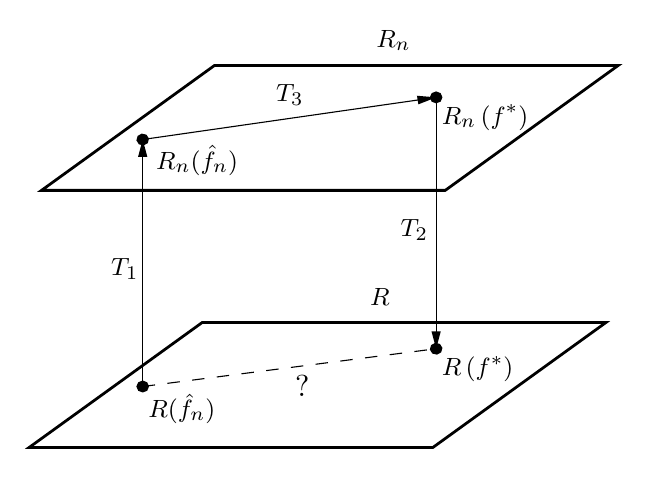
\begin{tikzpicture}[x=0.75pt,y=0.75pt,yscale=-0.7,xscale=0.75]
%uncomment if require: \path (0,503); %set diagram left start at 0, and has height of 503

%Shape: Parallelogram [id:dp6379841658274947] 
\draw  [line width=1]  (250.15,328) -- (509.5,328) -- (398.35,414) -- (139,414) -- cycle ;
%Shape: Parallelogram [id:dp5659534429170581] 
\draw  [line width=1]  (258.15,151) -- (517.5,151) -- (406.35,237) -- (147,237) -- cycle ;
%Straight Lines [id:da458543701942727] 
\draw    (212,372) -- (212,204) ;
\draw [shift={(212,202)}, rotate = 450] [fill={rgb, 255:red, 0; green, 0; blue, 0 }  ][line width=0.08]  [draw opacity=0] (12,-3) -- (0,0) -- (12,3) -- cycle    ;
\draw [shift={(212,372)}, rotate = 270] [color={rgb, 255:red, 0; green, 0; blue, 0 }  ][fill={rgb, 255:red, 0; green, 0; blue, 0 }  ][line width=0.75]      (0, 0) circle [x radius= 3.35, y radius= 3.35]   ;
%Straight Lines [id:da6580046139798694] 
\draw    (212,202) -- (398.52,173.3) ;
\draw [shift={(400.5,173)}, rotate = 531.25] [fill={rgb, 255:red, 0; green, 0; blue, 0 }  ][line width=0.08]  [draw opacity=0] (12,-3) -- (0,0) -- (12,3) -- cycle    ;
\draw [shift={(212,202)}, rotate = 351.25] [color={rgb, 255:red, 0; green, 0; blue, 0 }  ][fill={rgb, 255:red, 0; green, 0; blue, 0 }  ][line width=0.75]      (0, 0) circle [x radius= 3.35, y radius= 3.35]   ;
%Straight Lines [id:da5733317875250146] 
\draw    (400.5,173) -- (400.5,344) ;
\draw [shift={(400.5,346)}, rotate = 270] [fill={rgb, 255:red, 0; green, 0; blue, 0 }  ][line width=0.08]  [draw opacity=0] (12,-3) -- (0,0) -- (12,3) -- cycle    ;
\draw [shift={(400.5,173)}, rotate = 90] [color={rgb, 255:red, 0; green, 0; blue, 0 }  ][fill={rgb, 255:red, 0; green, 0; blue, 0 }  ][line width=0.75]      (0, 0) circle [x radius= 3.35, y radius= 3.35]   ;
%Straight Lines [id:da12727382381339924] 
\draw  [dash pattern={on 4.5pt off 4.5pt}]  (212,372) -- (400.5,346) ;
\draw [shift={(400.5,346)}, rotate = 352.15] [color={rgb, 255:red, 0; green, 0; blue, 0 }  ][fill={rgb, 255:red, 0; green, 0; blue, 0 }  ][line width=0.75]      (0, 0) circle [x radius= 3.35, y radius= 3.35]   ;

% Text Node
\draw (360.35,125.4) node [anchor=north west][inner sep=0.75pt]    {$R_{n}$};
% Text Node
\draw (356.35,302.4) node [anchor=north west][inner sep=0.75pt]    {$R$};
% Text Node
\draw (214,375.4) node [anchor=north west][inner sep=0.75pt]    {$R(\hat{f}_{n})$};
% Text Node
\draw (219,204.4) node [anchor=north west][inner sep=0.75pt]    {$R_{n}(\hat{f}_{n})$};
% Text Node
\draw (402.5,176.4) node [anchor=north west][inner sep=0.75pt]    {$R_{n}\left( f^{*}\right)$};
% Text Node
\draw (402.5,349.4) node [anchor=north west][inner sep=0.75pt]    {$R\left( f^{*}\right)$};
% Text Node
\draw (308.25,362.4) node [anchor=north west][inner sep=0.75pt]  [font=\large]  {$?$};
\draw (190,282.4) node [anchor=north west][inner sep=0.75pt]    {$T_{1}$};
% Text Node
\draw (376,255.4) node [anchor=north west][inner sep=0.75pt]    {$T_{2}$};
% Text Node
\draw (296,162.4) node [anchor=north west][inner sep=0.75pt]    {$T_{3}$};
\end{tikzpicture}
\vspace{1em}

\caption{\textbf{Figure}: Risk decomposition (well-specified)}
\end{center}

\subsection{The Mis-specification Case}
We call the problem mis-specification, when $f^* \not\in \mathcal{F}$.
\begin{theorem}[Bias-variance trade-off]
The excess risk $R(\hat{f}) - R(f^*)$ can be decomposed into 
\begin{align*} 
R(\widehat{f}_{n})-R\left(f^{\star}\right)=\underbrace{R(\widehat{f}_{n})-R\left(f^{\star, \mathcal{F}}\right)}_{\text {"Variance" }}+\underbrace{R\left(f^{\star, \mathcal{F}}\right)-R\left(f^{\star}\right)}_{\text {"Bias" }=\text { "approx error" }}
\end{align*}
where $f^{\star, \mathcal{F}} = \arg\min_{f\in\mathcal{F}} R(f)$.
\end{theorem}
\textbf{Remark}: The following figure provides some insights.
\begin{center}
    \tikzset{every picture/.style={line width=0.75pt}} %set default line width to 0.75pt        

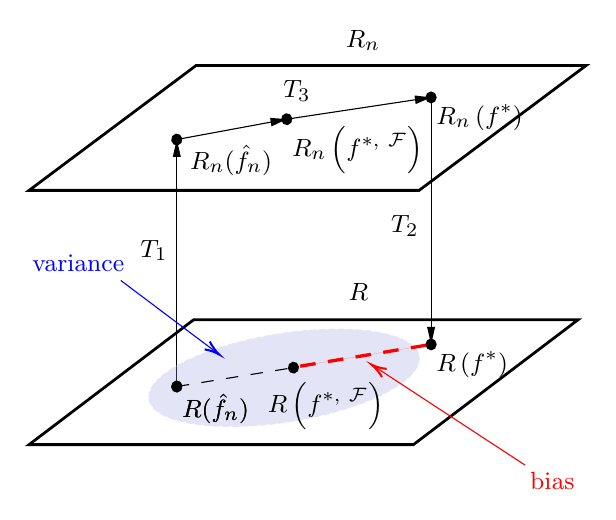
\begin{tikzpicture}[x=0.75pt,y=0.75pt,yscale=-0.7,xscale=0.65]
%uncomment if require: \path (0,428); %set diagram left start at 0, and has height of 428

%Shape: Parallelogram [id:dp7274687411777527] 
\draw  [line width=1]  (211.6,259) -- (496.5,259) -- (374.4,345) -- (89.5,345) -- cycle ;
%Shape: Parallelogram [id:dp5477732282695964] 
\draw  [line width=1]  (213.4,84) -- (502.5,84) -- (378.6,170) -- (89.5,170) -- cycle ;
%Straight Lines [id:da2018530395235334] 
\draw    (199,305) -- (199,137) ;
\draw [shift={(199,135)}, rotate = 450] [fill={rgb, 255:red, 0; green, 0; blue, 0 }  ][line width=0.08]  [draw opacity=0] (12,-3) -- (0,0) -- (12,3) -- cycle    ;
\draw [shift={(199,305)}, rotate = 270] [color={rgb, 255:red, 0; green, 0; blue, 0 }  ][fill={rgb, 255:red, 0; green, 0; blue, 0 }  ][line width=0.75]      (0, 0) circle [x radius= 3.35, y radius= 3.35]   ;
%Straight Lines [id:da7590655674070557] 
\draw    (199,135) -- (278.53,121.34) ;
\draw [shift={(280.5,121)}, rotate = 530.25] [fill={rgb, 255:red, 0; green, 0; blue, 0 }  ][line width=0.08]  [draw opacity=0] (12,-3) -- (0,0) -- (12,3) -- cycle    ;
\draw [shift={(199,135)}, rotate = 350.25] [color={rgb, 255:red, 0; green, 0; blue, 0 }  ][fill={rgb, 255:red, 0; green, 0; blue, 0 }  ][line width=0.75]      (0, 0) circle [x radius= 3.35, y radius= 3.35]   ;
%Straight Lines [id:da94095897726301] 
\draw    (387.5,106) -- (387.5,274) ;
\draw [shift={(387.5,276)}, rotate = 270] [fill={rgb, 255:red, 0; green, 0; blue, 0 }  ][line width=0.08]  [draw opacity=0] (12,-3) -- (0,0) -- (12,3) -- cycle    ;
\draw [shift={(387.5,106)}, rotate = 90] [color={rgb, 255:red, 0; green, 0; blue, 0 }  ][fill={rgb, 255:red, 0; green, 0; blue, 0 }  ][line width=0.75]      (0, 0) circle [x radius= 3.35, y radius= 3.35]   ;
%Straight Lines [id:da1976293015627566] 
\draw    (280.5,121) -- (385.52,106.28) ;
\draw [shift={(387.5,106)}, rotate = 532.02] [fill={rgb, 255:red, 0; green, 0; blue, 0 }  ][line width=0.08]  [draw opacity=0] (12,-3) -- (0,0) -- (12,3) -- cycle    ;
\draw [shift={(280.5,121)}, rotate = 352.02] [color={rgb, 255:red, 0; green, 0; blue, 0 }  ][fill={rgb, 255:red, 0; green, 0; blue, 0 }  ][line width=0.75]      (0, 0) circle [x radius= 3.35, y radius= 3.35]   ;
%Shape: Ellipse [id:dp35271263746573145] 
\draw  [color={rgb, 255:red, 255; green, 255; blue, 255 }  ,draw opacity=1 ][fill={rgb, 255:red, 152; green, 157; blue, 223 }  ,fill opacity=0.27 ][dash pattern={on 0.84pt off 2.51pt}] (185.95,299) .. controls (207.74,280.32) and (266.84,265.18) .. (317.95,265.18) .. controls (369.06,265.18) and (392.84,280.32) .. (371.05,299) .. controls (349.26,317.68) and (290.16,332.82) .. (239.05,332.82) .. controls (187.94,332.82) and (164.16,317.68) .. (185.95,299) -- cycle ;
%Straight Lines [id:da7033382741571668] 
\draw  [dash pattern={on 4.5pt off 4.5pt}]  (199,305) -- (285.5,292) ;
\draw [shift={(285.5,292)}, rotate = 351.45] [color={rgb, 255:red, 0; green, 0; blue, 0 }  ][fill={rgb, 255:red, 0; green, 0; blue, 0 }  ][line width=0.75]      (0, 0) circle [x radius= 3.35, y radius= 3.35]   ;
\draw [shift={(199,305)}, rotate = 351.45] [color={rgb, 255:red, 0; green, 0; blue, 0 }  ][fill={rgb, 255:red, 0; green, 0; blue, 0 }  ][line width=0.75]      (0, 0) circle [x radius= 3.35, y radius= 3.35]   ;
%Straight Lines [id:da46898574266560433] 
\draw [color={rgb, 255:red, 255; green, 0; blue, 0 }  ,draw opacity=1 ][fill={rgb, 255:red, 255; green, 0; blue, 0 }  ,fill opacity=1 ][line width=1.2]  [dash pattern={on 5.63pt off 4.5pt}]  (290.5,291) -- (387.5,276) ;
%Straight Lines [id:da534934643638076] 
\draw    (387.5,276) ;
\draw [shift={(387.5,276)}, rotate = 0] [color={rgb, 255:red, 0; green, 0; blue, 0 }  ][fill={rgb, 255:red, 0; green, 0; blue, 0 }  ][line width=0.75]      (0, 0) circle [x radius= 3.35, y radius= 3.35]   ;
%Straight Lines [id:da8410108610917204] 
\draw [color={rgb, 255:red, 255; green, 0; blue, 0 }  ,draw opacity=1 ]   (457,359) -- (345.21,291.04) ;
\draw [shift={(343.5,290)}, rotate = 391.3] [color={rgb, 255:red, 255; green, 0; blue, 0 }  ,draw opacity=1 ][line width=0.75]    (10.93,-3.29) .. controls (6.95,-1.4) and (3.31,-0.3) .. (0,0) .. controls (3.31,0.3) and (6.95,1.4) .. (10.93,3.29)   ;
%Straight Lines [id:da6689238100303159] 
\draw [color={rgb, 255:red, 0; green, 0; blue, 255 }  ,draw opacity=1 ]   (157.5,232) -- (228.86,281.85) ;
\draw [shift={(230.5,283)}, rotate = 214.94] [color={rgb, 255:red, 0; green, 0; blue, 255 }  ,draw opacity=1 ][line width=0.75]    (10.93,-3.29) .. controls (6.95,-1.4) and (3.31,-0.3) .. (0,0) .. controls (3.31,0.3) and (6.95,1.4) .. (10.93,3.29)   ;

% Text Node
\draw (322.35,58.4) node [anchor=north west][inner sep=0.75pt]    {$R_{n}$};
% Text Node
\draw (324.35,232.4) node [anchor=north west][inner sep=0.75pt]    {$R$};
% Text Node
\draw (201,308.4) node [anchor=north west][inner sep=0.75pt]    {$R(\hat{f}_{n})$};
% Text Node
\draw (207,137.4) node [anchor=north west][inner sep=0.75pt]    {$R_{n}(\hat{f}_{n})$};
% Text Node
\draw (389.5,109.4) node [anchor=north west][inner sep=0.75pt]    {$R_{n}\left( f^{*}\right)$};
% Text Node
\draw (389.5,279.4) node [anchor=north west][inner sep=0.75pt]    {$R\left( f^{*}\right)$};
% Text Node
\draw (282.5,124.4) node [anchor=north west][inner sep=0.75pt]    {$R_{n}\left( f^{*,\ \mathcal{F}}\right)$};
% Text Node
\draw (264.5,300.4) node [anchor=north west][inner sep=0.75pt]    {$R\left( f^{*,\ \mathcal{F}}\right)$};
\draw (170,202.4) node [anchor=north west][inner sep=0.75pt]    {$T_{1}$};
% Text Node
\draw (356,185.4) node [anchor=north west][inner sep=0.75pt]    {$T_{2}$};
% Text Node
\draw (276,92.4) node [anchor=north west][inner sep=0.75pt]    {$T_{3}$};
% Text Node
\draw (459,362.4) node [anchor=north west][inner sep=0.75pt]  [color=red  ,opacity=1 ]  {$\color{red} \mathrm{bias}$};
% Text Node
\draw (201,308.4) node [anchor=north west][inner sep=0.75pt]    {$R(\hat{f}_{n})$};
% Text Node
\draw (90,212.4) node [anchor=north west][inner sep=0.75pt]  [color=blue  ,opacity=1 ]  {$\color{blue} \mathrm{variance}$};
\end{tikzpicture}

\caption{\textbf{Figure}: Bias and variance under mis-specification}
\end{center}


\section{Concentration bounds (Ch. 2)}
\subsection{Classical bounds}
The most basic tail bound is Markov's inequality.
\begin{theorem}[Markov's inequality]
For a random non-negative variable $X$ with finite mean,
\begin{align*}
    P(X \geq t) \leq \frac{\mathbb{E} X}{t}, \qquad \forall t > 0.
\end{align*}
\end{theorem}
\begin{proof} Using the non-negativity of $X$ and the definition of expectation,
\begin{align*}
     \mathbb{E}X & =\int_0^\infty x f(x) \d x = \int _{0}^{t}xf(x)\d x+\int_{t}^{\infty }xf(x) \d x \\
     & \geq \int_{t}^{\infty }xf(x)\d x\geq t \int _{a}^{\infty}f(x)\d x  = t P(X\geq t).
\end{align*}
\end{proof}

\begin{theorem}[Chebyshev's inequality]
For a random variable $X$ with finite $k$-th order center momentum,
\begin{align*}
    P(|X - \mu| \geq t) & = P(|X - \mu|^k \geq t^k) \\
    & \leq \frac{\mathbb{E} |X - \mu|^k}{t^k}, \qquad \forall t > 0.
\end{align*}
\end{theorem}
\begin{proof} Replacing $X$ with $|X - \mu|^k$ in Markov's inequality.
\end{proof}

\begin{method}[Chernoff bound] Apply Markov's inequality to random variable $Y = e^{\lambda (X - \mu)}$ ($0 \leq \lambda \leq b$), we get
\begin{align*}
    P(X - \mu \geq t) = P(e^{\lambda (X - \mu)} \geq e^{\lambda t}) \leq \frac{\EE{e^{\lambda(X - \mu)}}}{e^{\lambda t}}.
\end{align*}
Then, optimizing $\lambda$ to get a tighter bound,
\begin{align*}
    \log  P(X - \mu \geq t) \leq \inf_{\lambda} \left( \log \EE{e^{\lambda(X - \mu)}} - \lambda t \right).
\end{align*}
\end{method}
Chernoff bound will be used in achieving tail bounds of the sub-Gaussian and sub-exponential distribution.

\subsection{Sub-Gaussian and Hoeffding bounds}
\begin{definition}[Sub-Gaussian] A random variable $X$ with mean $\mu$ is sub-Gaussian with parameter $\siamg$ if one of following holds:
\begin{itemize}
    \item MGF condition: $$\EE{e^{\lambda (X - \mu)} \leq e^{\frac{\lambda^2 \sigma^2 }{2}}}, \quad \forall \lambda \in \R.$$
    \item Tail bound condition ($Z \sim \NN(0, \sigma^2)$): $$P(|X - \mu| \geq t) \leq c P(|Z - \mu| \geq t), \quad \exists c > 0, \forall t \geq 0.$$
\end{itemize}
\end{definition}
\noindent For simplicity, we denote the sub-Gaussian random variable $X$ with mean $\mu$ and parameter $\sigma^2$ as $X \sim SG(\mu, \sigma^2)$.

\begin{property}[Sub-Gaussian tail bound\label{prop:sub-gaussian-tail}] For $X \sim SG(\mu, \sigma^2)$,
\begin{align*}
    P(X - \mu \geq t) \leq e^{-\frac{t^2}{2\sigma^2}}, \quad \forall t \in \R.
\end{align*}
\end{property}
\begin{proof}
Applying Chernoff bound on $e^{\lambda(X - \mu)}$, we have
\begin{align*}
    \log  P(X - \mu \geq t) & \leq \inf_{\lambda > 0} \left( \log \EE{e^{\lambda(X - \mu)}} - \lambda t \right) \\
    & \leq  \inf_{\lambda > 0} \left(\frac{\sigma^2 \lambda^2}{2}- \lambda t \right) = -\frac{t^2}{2 \sigma^2}.
\end{align*}
Taking exponential on both sides gives the desired form.
\end{proof}

\begin{property}[Sum of sub-Gaussian RVs\label{prop:sum_sub_gaussian}] For $X_1 \sim SG(\mu_1, \sigma_1^2)$, $X_2 \sim SG(\mu_2, \sigma_2^2)$, 
\begin{align*}
    X_1 + X_2 \sim SG(\mu_1 + \mu_2, \sigma_1^2 + \sigma_2^2).
\end{align*}
\end{property}

\begin{property}[Sub-Gaussian for bounded RV]
For a RV $X \in [a, b]$ almost surely, $X$ is a sub-Gaussian with parameter at most $\sigma = \frac{b-a}{2}$.
\end{property}
\begin{proof}
Define function $\phi(\lambda) = \log \EE e^{\lambda x}$. It is easy to show that $\phi(0) = 0$ and $\phi'(0) = \EE X := \mu$. The second derivative is 
$$
\phi''(\lambda) = \EE_\lambda[X^2] -  \EE_\lambda[X]^2, \quad \text{where}\ \EE_\lambda[X] = \frac{\EE f(X) e^{\lambda X}}{\EE e^{\lambda X}} 
$$
Taking a Taylor expansion of $\phi(\lambda)$ at $\lambda=0$,
\begin{align*}
    \phi(\lambda) & =\phi(0) + \lambda \phi'(0) + \frac{\lambda^2}{2} \phi''(\epsilon) \\
    & \leq \lambda \mu + \frac{\lambda^2}{2} - \frac{(b-a)^2}{4}.
\end{align*}
\end{proof}

\begin{theorem}[Hoeffding bound] For $n$ independent sub-Gaussian random variables $X_i \in SG(\mu_i, \sigma_i^2), i = [n]$, 
\begin{align*}
    P\left(\sum_{i=1}^n (X_i - \mu_i) \geq t \right) \leq e^{-\frac{t^2}{2 \sum_{i=1}^n \sigma_i^2}}
\end{align*}
\end{theorem}
\begin{proof}
Using the sub-Gaussian tail bound (Prop.~\ref{prop:sub-gaussian-tail}) and the property of sum of Sub-Gaussian RVs (Prop.~\ref{prop:sum_sub_gaussian}).
\end{proof}

\begin{theorem}[Sub-Gaussian maxima\label{thm:sub-gaussian-maxima}]
For a sequence of sub-Gaussian RVs $\{X_i\}_{i=1}^n$, $X_i \sim SG(0, \sigma^2)$, the following bounds hold,
\begin{align*}
    \mathbb{E} \max _{i=1, \ldots, n} X_{i} & \leq \sqrt{2\sigma^{2} \log n}\\
    \mathbb{E} \max _{i=1, \ldots, n} |X|_{i} & \leq \sqrt{2 \sigma^{2} \log 2n}
\end{align*}
\end{theorem}
\textbf{Remark}: This bound is frequently used in deriving other bounds.

\begin{proof}
Let $f(x) = e^{\lambda x}$ ($\lambda > 0$), we have
	\begin{align*}
		e^{\lambda \EE[\max_i X_i]} & \leq \EEE{e^{\lambda \max_i X_i}} \qquad (f(x) \text{ is convex})\\
		& = \EEE{\max_i e^{\lambda X_i}} \qquad (f(x) \text{ is mono-increasing}) \\
		& \leq \sum_{i=1}^n \EEE{e^{\lambda X_i}} \leq n e^{\sigma^2 \lambda^2 / 2} 
	\end{align*}
	Therefore, 
	\begin{align*}
		\EE[\max_i X_i] \leq \frac{\log n}{\lambda} + \frac{\lambda \sigma^2}{2}, \quad \forall \lambda > 0.
	\end{align*}
	Using Chernoff bound, we get
	\begin{align*}
		\EE[\max_i X_i] \leq \inf_{\lambda>0} \frac{\log n}{\lambda} + \frac{\lambda \sigma^2}{2}  = \sqrt{2\sigma^{2} \log n},
	\end{align*}

The second inequality can be proved by using the fact that
	\begin{align*}
		\max_i |X_i| = \max \left\{ X_1, \cdots, X_n, (-X_1). \cdots, (-X_n) \right\}.
	\end{align*}
\end{proof}

\subsection{Sub-exponential and Bernstein bounds}
\begin{definition}[Sub-exponential] A random variable $X$ with mean $\mu$ is sub-exponential with parameter $(v, \alpha)$ if one of following holds:
\begin{itemize}
\setlength{\itemsep}{-0.5em}
    \item MGF condition: $$\EE{e^{\lambda (X - \mu)} \leq e^{\frac{\lambda^2 v^2}{2}}}, \quad \forall |\lambda| < \frac{1}{\alpha}.$$
    \item Tail bound condition: $$P(|X - \mu| \geq t) \leq c_1 e^{-c_2 t}, \quad \exists c_1, c_2 > 0, \forall t \geq 0.$$
\end{itemize}
\end{definition}

\begin{theorem}[Bernstein-type bound]For any random variable satisfying the Bernstein condition $\left|\mathbb{E}\left[(X-\mu)^{k}\right]\right| \leq \frac{1}{2} k ! \sigma^{2} b^{k-2}$, we have,
\begin{align*}
    P(|X-\mu| \geq t) \leq 2 e^{-\frac{t^{2}}{2\left(\sigma^{2}+b t\right)}}
\end{align*}
\end{theorem}
\textbf{Remark}: For bounded RV, this bound is more tighter compared with Hoeffding bound for sub-Gaussian with $\sigma$ when $\sigma << b$.

\begin{proof} Using Taylor expansion of the the MGF of sub-exponential RV, we have
\begin{align*}
\mathbb{E}\left[e^{\lambda(X-\mu)}\right] & \leq 1+\frac{\lambda^{2} \sigma^{2}}{2}+\sum_{k=3}^{\infty} \lambda^{k} \frac{\mathbb{E}\left[(X-\mu)^{k}\right]}{k !} \\
& \leq 1+\frac{\lambda^{2} \sigma^{2}}{2}+\frac{\lambda^{2} \sigma^{2}}{2} \sum_{k=3}^{\infty}(|\lambda| b)^{k-2} \\
& \leq 1+\frac{\lambda^{2} \sigma^{2} / 2}{1-b|\lambda|} \leq e^{\frac{\lambda^{2} \sigma^{2} / 2}{1-b|\lambda|}}
\end{align*}
Then, based on Chernoff bound, we get
\begin{align*}
\log  P(X - \mu \geq t) & \leq \inf_{\lambda} \left( \log \EE{e^{\lambda(X - \mu)}} - \lambda t \right) \\
& \leq \inf_{\lambda}\left(\frac{\lambda^{2} \sigma^{2} / 2}{1-b|\lambda|} - \lambda t  \right) =  -\frac{t^{2}}{2\left(\sigma^{2}+b t\right)}.
\end{align*}
This gives the one-side bound. The two-side version can be obtained with additional factor of 2.
\end{proof}

\subsection{Martingale-based Methods}
\begin{definition}[Martingale]
A sequence of RVs $Y_1, Y_2, \cdots$ is said to be a martingale with respect to another sequence of RVs $X_1, X_2, ...$ if for all $n$,
\begin{align*}
    \mathbb{E} \vert Y_{n}\vert < \infty \quad \text{and} \quad \mathbb{E} [Y_{n+1}\mid X_{1},\ldots ,X_{n}] = Y_{n}.
\end{align*}

\end{definition}

\begin{definition}[Doob martingale difference] 
For a function $g_n: \mathcal{X} \rightarrow \R$ on independent RV $X_i \in \mathcal{X}$ and the $\sigma$-field $F_i = \sigma(X_1, \cdots, X_i)$, the Doob martingale difference $\{(D_i, F_i)\}_{i=1}^n$ is defined as
\begin{align*}
    D_i := S_i - S_{i-1},\quad \text{where } S_i := \mathbb{E}[g_n(X) \mid X_1, \cdots, X_i]
\end{align*}
\end{definition}
Here, we often define $S_0 = \EE[g_n(X)]$, so that we have the \textit{telescoping decomposing}
\begin{align*}
    S_n - S_0 = \sum_{i=1}^n D_i.
\end{align*}

\begin{theorem}[Azuma-Hoeffding]
For a martingale difference sequence $\{(D_i, F_i)\}_{i=1}^n$, $D_i \mid F_{i-1} \in [a_i, b_i]$ almost surely for $i=[n]$, then
\begin{align*}
    P\left(\sum_{i=1}^n D_i \geq t\right) \leq e^{-\frac{2t^2}{\sum_{i=1}^n (b_i - a_i)^2}}
\end{align*}
\end{theorem}
\begin{proof}
Since $D_i \mid F_{i-1} \in [a_i, b_i]$, we have
\begin{align*}
    \EEE{e^{\lambda D_i} \mid F_{i-1}} \leq e^{\frac{\lambda^2 (b_i - a_i)^2}{8}}
\end{align*}
To show the $\sum_{i=1}^n D_i$ is sub-Gaussian, we use the iterated expectation as, 
\begin{align*}
 \EEE{e^{\lambda \sum_{i=1}^n D_i}}  = &\ \E{D_1, \cdots, D_{n}}{e^{\lambda \sum_{i=1}^{n-1} D_i} \cdot \E{D_n}{e^{\lambda D_n} \mid F_{n-1}}} \\
    = & \ \E{D_1, \cdots, D_{n-1}}{e^{\lambda \sum_{i=1}^{n-1} D_i}} \cdot \E{D_n}{e^{\lambda D_n} \mid F_{n-1}} \\
    \leq &\ \E{D_1, \cdots, D_{n-1}}{e^{\lambda \sum_{i=1}^{n-1} D_i}} e^{\frac{\lambda^2 (b_n - a_n)^2}{8}}
\end{align*}
Using it recursively, we get $\EEE{e^{\lambda \sum_{i=1}^n D_i}} \leq e^{\frac{\lambda^2 \sum_{i=1}^n (b_i - a_i)^2}{8}}$. Then we can achieve the desired bound via Chernoff bound (similar to Prop.~\ref{prop:sub-gaussian-tail}, sub-Gaussian tail bound).
\end{proof}

\begin{theorem}[McDiarmid inequality]
If $g_n(Z)$ satisfies the bounded difference condition, i.e. $|g_n(z) - g_n(z^{\backslash k})| \leq \sigma_k$,  for a random vector $Z$ with $n$ independent entries, then
\begin{align*}
    P(g_n(Z) - \EE g_n(Z) \geq t) \leq e^{-\frac{2t^2}{\sum_{i=1}^n \sigma^2_i}}
\end{align*}
where $z = (z_1, \cdots, z_k, \cdots, z_n)$, $z^{\backslash k} = (z_1, \cdots, z'_k, \cdots, z_n)$.
\end{theorem}
\begin{proof}
First, please note that
$$ g_n(Z) - \EE g_n(Z) = S_n - S_0 = \sum_{i=1}^n D_i,
$$
where $D_i = \mathbb{E}\left[g_{n}(Z) \mid Z_{1}, \ldots, Z_{i}\right]-\mathbb{E}\left[g_{n}(Z) \mid Z_{1}, \ldots, Z_{i-1}\right]$.
Therefore, we can use the Azuma-Hoeffding inequality if we show that $D_i$ is bounded.
\begin{align*}
    D_k & \leq  \sup _{z} \mathbb{E}_{Z_{k+1:n}}\left[g_n\left(Z_{1:k-1}, z, Z_{k+1:n}\right)\right] \\
        & \qquad  -\inf_{z} \mathbb{E}_{Z_{k+1:n}}\left[g_n\left(Z_{1:k-1}, z, Z_{k+1:n}\right)\right] \\
    & \leq \sup _{z, z'} \bigg|\, \mathbb{E}_{Z_{k+1:n}}\left[g_n\left(Z_{1:k-1}, z, Z_{k+1:n}\right)\right]  \\
    & \qquad - \mathbb{E}_{Z_{k+1:n}}\left[g_n\left(Z_{1:k-1}, z',  Z_{k+1:n}\right)\right] \bigg| \\
    & \leq \sigma_k
\end{align*}
Then, we can plug it into the Azuma-Hoeffding inequality and conclude the proof.
\end{proof}

\subsection{Functional bounds}
\begin{theorem}[Lipschitz functions]
If $g: \R^n \rightarrow \R$ is $L$-Lipschitz function for vector $z$ with edclidean norm, $z_i \sim \NN(0, \sigma^2)$. 
$$
P(g(z)-\mathbb{E} g(z) \geq t) \leq e^{-\frac{c t^{2}}{L^{2} \sigma^{2}}}
$$
\end{theorem}
\section{Uniform Laws of Large Numbers {(Ch.~4)}}
\subsection{Motivation}
\begin{definition}[Glivenko-Cantelli class]
We say $\mathcal{F}$ is Glivenko-Cantelli class if
$$ \norm{P_n - P}_{\mathcal{F}} := \sup_{f \in \mathcal{F}} \bigg| \frac{1}{n} \sum_{i=1}^n f(X_i) - \EE f(X_i) \bigg| \longrightarrow 0,
$$
in probability as $n \rightarrow 0$.
\end{definition}
\subsection{A uniform law via Rademacher complexity}
\begin{theorem}[Uniform law of large number] For $b$-uniformly bounded $\mathcal{F}$, we have
\begin{align*}
    P\left(\sup_{f\in \mathcal{F}} R(f) - R_n(f) \geq 2 \mathcal{R}_n(\mathcal{F}) + t\right) \leq e^{-\frac{nt^2}{2b^2}}.
\end{align*}
Here, population risk is $R(f) = \mathbb{E} f(x)$ and empirical risk is $R_n(f) = \frac{1}{n} \sum_{i=1}^n f(x_i)$. The Rademacher complexity is
\begin{align*}
    \mathcal{R}_{n}(\mathcal{F})=\mathbb{E}_{\epsilon} \sup _{h \in \mathcal{H}} \frac{1}{n} \sum_{i=1}^{n} \epsilon_{i} h(z_i), \quad \epsilon_i \sim \mathrm{Red}(\{-1, 1\})
\end{align*}
\end{theorem}
\begin{proof}
1. \textbf{Concentration around mean}. Let's denote
$$g_n(x_{1:n}) :=   \sup_{f \in \mathcal{F}} R(f) - R_n(f)= \sup_{f \in \mathcal{F}} \frac{1}{n} \sum_{i=1}^n f(x_i) - \EE{f(x)}.$$
Let $z = (x_1, \cdots, x_k, \cdots, x_n)$ and $z^{\backslash k} = (x_1, \cdots, x'_k, \cdots, x_n)$,
\begin{align*}
& \left|g_{n}(z)-g_{n}\left(z^{\backslash k}\right)\right| \\
= & \left|\sup _{h \in \mathcal{H}} \frac{1}{n} \sum_{i}\left[h\left(z_{i}\right)-\mathbb{E} h\right]-\sup _{\tilde{h} \in \mathcal{H}} \frac{1}{n} \sum_{i}\left[\tilde{h}\left(z_{i}^{\backslash k}\right)-\mathbb{E} \tilde{h}\right]\right| \\
\leq & \left|\sup _{h \in \mathcal{H}} \frac{\sum_{i} h\left(z_{i}\right)-h\left(z_{i}^{\backslash k}\right)}{n}\right| \leq\left|\sup _{h \in \mathcal{H}} \frac{h\left(x_{k}\right)-h\left(x_{k}^{\prime}\right)}{n}\right| \leq \frac{2 b}{n},
\end{align*}
which means $g_n$ has Lipschitz property.
Using McDiarmid inequality, $P\left(g_{n}(X) - \mathbb{E}g_{n}(X) \geq t\right) \leq e^{-\frac{n t^{2}}{2 b^{2}}}$.


2. \textbf{Upper bound on mean}. Using symmetrization technique and the definition of Rademacher complexity, we have
\begin{align*}
    \mathbb{E} g_n(X) & = \E{X}{\sup_{f \in \mathcal{F}} \frac{1}{n} \sum_{i=1}^n f(x_i) - \EE{f(x)}} \\
    & \leq \E{X, Y}{\sup_{f \in \mathcal{F}} \frac{1}{n} \sum_{i=1}^n f(x_i) - f(y_i)} & (\text{symmetrize}) \\
    & = \E{X, Y, \epsilon}{\sup_{f \in \mathcal{F}} \frac{1}{n} \sum_{i=1}^n \epsilon (f(x_i) - f(y_i))} & (\text{plug in } \epsilon) \\
    & \leq 2 \E{X, \epsilon}{\sup_{f \in \mathcal{F}} \frac{1}{n} \sum_{i=1}^n \epsilon f(x_i)} = 2 \mathcal{R}_n(\mathcal{F}).
\end{align*}
Combining these two parts, we have the desired theorem that $P\left(g_{n}(X) - 2\mathcal{R}_n(\mathcal{F}) \geq t\right) \leq e^{-\frac{n t^{2}}{2 b^{2}}}$.
\end{proof}

\begin{theorem}[Uniform law - corollary] If $\mathcal{R}_n(\mathcal{F}) = o(1)$, then when $n \rightarrow \infty$, we have
\begin{align*}
    \sup_{f\in \mathcal{F}} R(f) - R_n(f) \longrightarrow 0, \quad (a.s.)
\end{align*}
In other words, $\mathcal{R}_n(\mathcal{F}) = o(1)$ implies that $\mathcal{F}$ is a Glivenko-Cantelli class.
\end{theorem}
\begin{proof}
Let $\mathcal{E}_n(\alpha)$ denote the event that $\sup_{f\in \mathcal{F}} R(f) - R_n(f) \geq \alpha$. The uniform law shows that
\begin{align*}
    P\left(\mathcal{E}_n( 2\mathcal{R}_n(\mathcal{H}) + t )\right) & \leq  e^{-\frac{nt^2}{2b^2}}.
\end{align*}
Using union bound,  $\forall t > 0$, we have,
\begin{align*}
   \sum_{n=1}^{\infty} P(\mathcal{E}_n(2t)) & \leq \sum_{n=1}^{k} P\left(\mathcal{E}_n\left(2t\right)\right)  + \sum_{n=k+1}^\infty P\left(\mathcal{E}_n\left(2\mathcal{R}_n(\mathcal{H}) + t \right)\right) \\
    & \leq \sum_{n=1}^{k} P\left(\mathcal{E}_n\left(2t\right)\right) + \sum_{n=k+1}^\infty  e^{-\frac{nt^2}{2b^2}} < \infty.
\end{align*}
The $k$ is chosen such that when $n > k$, $\mathcal{R}_n(f) < \frac{t}{2}$. Such $k$ must exist, since $\mathcal{R}_n(f) = o(1)$.
Using the Borel-Cantalli lemma, we show that
\begin{align*}
    P\left(\lim_{n \rightarrow \infty} \sup \mathcal{E}_n(2t) \right) = 0.
\end{align*}
Considering that $t$ can be arbitrarily small, we have
\begin{align*}
    P\left(\lim_{n \rightarrow \infty} \sup_{f\in \mathcal{F}} R(f) - R_n(f) = 0 \right) = 1.
\end{align*}
\end{proof}

\subsection{Upper bounds on the Rademacher complexity}
\begin{definition}[Growth function]
The growth function $N_\mathcal{H}$ for a hypothesis space $\mathcal{H}$ is defined as: $\forall m \in \mathbb{N}$,
\begin{align*}
    N_{\mathcal{H}}(n) := \sup_{z_{1:n} \subseteq Z }\left|\left\{\left(h\left(z_{1}\right), \cdots, h\left(z_{n}\right)\right) \mid h \in \mathcal{H}\right\}\right|
\end{align*}
\end{definition}
\textbf{Remark}: Growth function measures the maximum number of distinct ways in which m points can be classified using hypotheses in $\mathcal{H}$.

\begin{theorem}[Massart lemma]
For a data set $z_{1:n} = \{z_1, \cdots, z_n\}$, the hypothesis $h: Z \rightarrow\{0,1\}$ and the hypothesis space $\mathcal{H}(z_{1:n}):=\{(h(z_1), \cdots, h(z_n)) \mid h \in \mathcal{H}\}$, we have
\begin{align*}
    {\mathcal{R}}_{n}\left(\mathcal{H}\right):=\mathbb{E}_{\epsilon}\left[ \sup _{h \in \mathcal{H}} \frac{1}{n} \sum_{i=1}^{n} \epsilon_{i} h\left(z_{i}\right)\right] \leq 2 \sqrt{\frac{\log \left|\mathcal{H}\left(z_{1:n}\right)\right|}{n}}
\end{align*}
\end{theorem}
\textbf{Remark}: Using this result, we can now bound the Rademacher complexity in terms of the growth function.

\vspace{1em}
\begin{proof}
First, we show that $\epsilon^T \theta$ is $\sqrt{n}$ sub-Gaussian. Using the independence of $z$, $\forall \lambda \in \mathbb{R}$, we have
\begin{align*}
\mathbb{E}_\epsilon \left[ \exp(\lambda \epsilon^\top\theta)\right] & = \mathbb{E}_\epsilon \left[\exp \left( \lambda \sum_{i=1}^n \epsilon_i \theta_i \right) \right] \\
& = \mathbb{E}_{\epsilon_1} \left[\exp \left(\lambda\epsilon_1 \theta_1 \right) \right] \cdots \mathbb{E}_{\epsilon_n} \left[\exp \left(\lambda \epsilon_n \theta_n \right) \right]\\
& \leq \exp\left(\frac{\lambda^2 \theta_1^2}{2} + \cdots + \frac{\lambda^2 \theta_n^2}{2} \right) \leq \exp\left(\frac{\lambda^2 n}{2}\right).
\end{align*}
Next, using the Gaussian maxima, we get
\begin{align*}
    \mathbb{E} \max _{\theta \in \mathbb{T}} \epsilon^T \theta \leq 2 \sqrt{n \log \left|\mathcal{H}\left(z_{1}^{n}\right)\right|}
\end{align*}
Then, we can get the intended results.
\end{proof}

\begin{definition}[VC Dimension]
The VC dimension of $\mathcal{H}$ is  the biggest $n \in \mathbb{N}$ such that there exists $n$ samples in $\mathcal{H}$ which can be arbitrarily scattered by a binary classifier, i.e.,
\begin{align*}
    d_{VC} = \max_{n \in \mathbb{N}} n, \quad \text{s.t. } \exists z_{1:n} \in Z^n, \mathcal{H}(z_{1:n}) = \{0,1\}^n.
\end{align*}
Here, $\mathcal{H}(z_{1:n}):=\{(h(z_1), \cdots, h(z_n)) \mid h \in \mathcal{H}\}$。
\end{definition}
\textbf{Remark}: Finite VC dimension can make $\mathcal{H}$ a Glivenko-Cantelli class.

\begin{theorem}[Sauer-Shelah]
For a space $\mathcal{H}$ with VC dimension $d_{VC}$, for any $z_1, \cdots, z_n$, we have growth function
\begin{align*}
    N_\mathcal{H}(n) := \sup_{z_{1:n} \in Z^n} |\mathcal{H}(z_{1:n})| \leq (n + 1)^{d_{VC}}, \quad \forall n \geq d_{VC}
\end{align*}
\end{theorem}
\begin{proof}
Proof by combination algebra. See the Chapter 4.3 for more details.
\end{proof}

\begin{theorem}[Rademacher contraction]
For any $\mathbb{T} \subseteq \R^n$ and $\ell : \R^n \rightarrow \R^n$ with univariate $L$-Lipschitz
functions it holds that
\begin{align*}
    \tilde{\mathcal{R}}_{n}(\ell \circ \mathbb{T}) \leq L \tilde{\mathcal{R}}_{n}(\mathbb{T})
\end{align*}
\end{theorem}
\begin{proof}
See the slides of Lecture 5.
\end{proof}



\section{Non-uniform Learnability (Lec. 6-7)}

\subsection{Structural risk minimization (SRM)}
\begin{definition}[SRM]
Say we have a nested family of function spaces $\mathcal{H}_{1} \subset \mathcal{H}_{2} \subset \cdots$, where $\mathcal{H} = \bigcup_k \mathcal{H}_{k} $. For each $\mathcal{H}_k$ define the event
$$
E_{k, h}=\left\{R(h)-R_{n}(h) \leq c \sqrt{\frac{\log \left(1 / \delta_{k}\right)}{n}}+2 \mathcal{R}_{n}\left(\mathcal{H}_{k}\right)\right\}.
$$
\end{definition}

\begin{theorem}[Uniform law via the SRM]
Define $k(h) = \min \{k \mid f \in \mathcal{H}_k\}$ which for each $h$ finds the minimum set $\mathcal{H}_k$.

If $P(\bigcap_{h \in \mathcal{H}_k} E_{k, h} ) \geq 1 - \delta_k$ for each $k$ and if $\sum_k \delta_k \leq \delta$, with probability at least $1 - \delta$,
$$
\sup _{h \in \mathcal{H}} R(h)-R_{n}(h) \leq c \sqrt{\frac{\log \left(1 / \delta_{k(h)}\right)}{n}}+2 \mathcal{R}_{n}\left(\mathcal{H}_{k(h)}\right)
$$
\end{theorem}
\begin{proof}
Observe that
\begin{align*}
A := & \left\{\sup _{h \in \mathcal{H}} R(h)-R_{n}(h) \leq c \sqrt{\frac{\log \left(1 / \delta_{k(h)}\right)}{n}}+2 \mathcal{R}_{n}\left(\mathcal{H}_{k(h)}\right)\right\} \\
=& \cap_{h \in \mathcal{H}} \cap_{k: h \in \mathcal{H}_{k}} E_{k, h}=\cap_{k \in \mathbb{N}} \cap_{h \in \mathcal{H}_{k}} E_{k, h}
\end{align*}
Then, we can use the union bound,
\begin{align*}
    P(A)=1-P\left(\cup_{k \in \mathbb{N}} \cup_{h \in \mathcal{H}_{k}} E_{k, h}\right) \geq 1-\sum_{k} \delta_{k} \geq 1-\delta,
\end{align*}
which concludes the proof.
\end{proof}
\begin{center}
    \tikzset{every picture/.style={line width=0.75pt}} %set default line width to 0.75pt        

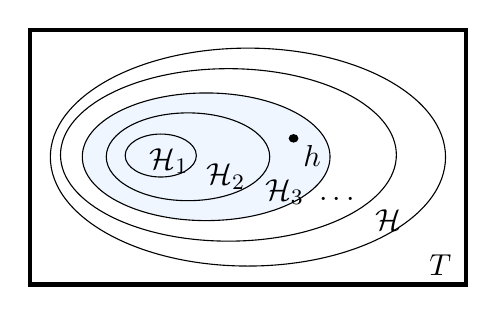
\begin{tikzpicture}[x=0.75pt,y=0.75pt,yscale=-0.6,xscale=0.7]
%uncomment if require: \path (0,365); %set diagram left start at 0, and has height of 365

%Shape: Circle [id:dp5556054645273254] 
\draw  [fill={rgb, 255:red, 0; green, 0; blue, 0 }  ,fill opacity=1 ] (376.28,140.87) .. controls (376.28,139.24) and (377.6,137.91) .. (379.24,137.91) .. controls (380.87,137.91) and (382.19,139.24) .. (382.19,140.87) .. controls (382.19,142.5) and (380.87,143.83) .. (379.24,143.83) .. controls (377.6,143.83) and (376.28,142.5) .. (376.28,140.87) -- cycle ;
%Shape: Rectangle [id:dp5281419369218745] 
\draw  [line width=1.5]  (197.67,47.75) -- (498,47.75) -- (498,252.25) -- (197.67,252.25) -- cycle ;
%Shape: Ellipse [id:dp5525274261812825] 
\draw   (218.84,148.25) .. controls (218.84,110) and (270.58,79) .. (334.42,79) .. controls (398.25,79) and (450,110) .. (450,148.25) .. controls (450,186.49) and (398.25,217.5) .. (334.42,217.5) .. controls (270.58,217.5) and (218.84,186.49) .. (218.84,148.25) -- cycle ;
%Shape: Ellipse [id:dp47565683667848213] 
\draw  [fill={rgb, 255:red, 239; green, 246; blue, 255 }  ,fill opacity=1 ] (233.84,149.75) .. controls (233.84,121.44) and (272,98.5) .. (319.09,98.5) .. controls (366.17,98.5) and (404.34,121.44) .. (404.34,149.75) .. controls (404.34,178.05) and (366.17,201) .. (319.09,201) .. controls (272,201) and (233.84,178.05) .. (233.84,149.75) -- cycle ;
%Shape: Ellipse [id:dp8225386024812087] 
\draw   (250.34,149.75) .. controls (250.34,130.28) and (275.52,114.5) .. (306.59,114.5) .. controls (337.65,114.5) and (362.84,130.28) .. (362.84,149.75) .. controls (362.84,169.22) and (337.65,185) .. (306.59,185) .. controls (275.52,185) and (250.34,169.22) .. (250.34,149.75) -- cycle ;
%Shape: Ellipse [id:dp012503998897681612] 
\draw   (263.34,148.75) .. controls (263.34,139.22) and (274.3,131.5) .. (287.84,131.5) .. controls (301.37,131.5) and (312.34,139.22) .. (312.34,148.75) .. controls (312.34,158.27) and (301.37,166) .. (287.84,166) .. controls (274.3,166) and (263.34,158.27) .. (263.34,148.75) -- cycle ;
%Shape: Ellipse [id:dp7411816000021694] 
\draw   (211.84,150) .. controls (211.84,101.67) and (272.72,62.5) .. (347.84,62.5) .. controls (422.95,62.5) and (483.84,101.67) .. (483.84,150) .. controls (483.84,198.32) and (422.95,237.5) .. (347.84,237.5) .. controls (272.72,237.5) and (211.84,198.32) .. (211.84,150) -- cycle ;
%Shape: Circle [id:dp06594432447625231] 
\draw  [fill={rgb, 255:red, 0; green, 0; blue, 0 }  ,fill opacity=1 ] (376.28,134.96) .. controls (376.28,133.33) and (377.6,132) .. (379.24,132) .. controls (380.87,132) and (382.19,133.33) .. (382.19,134.96) .. controls (382.19,136.59) and (380.87,137.91) .. (379.24,137.91) .. controls (377.6,137.91) and (376.28,136.59) .. (376.28,134.96) -- cycle ;

% Text Node
\draw (471,226.4) node [anchor=north west][inner sep=0.75pt]    {\large$T$};
% Text Node
\draw (278.5,140.9) node [anchor=north west][inner sep=0.75pt]    {\large $\mathcal{H}_{1}$};
% Text Node
\draw (317.5,153.4) node [anchor=north west][inner sep=0.75pt]    {\large$\mathcal{H}_{2}$};
% Text Node
\draw (358,165.9) node [anchor=north west][inner sep=0.75pt]    {\large$\mathcal{H}_{3}$};
% Text Node
\draw (395,176.4) node [anchor=north west][inner sep=0.75pt]    {\large$\cdots $};
% Text Node
\draw (434,189.9) node [anchor=north west][inner sep=0.75pt]    {\large$\mathcal{H}$};
% Text Node
\draw (384.19,138.36) node [anchor=north west][inner sep=0.75pt]    {\large$h$};
\end{tikzpicture}

\caption{\textbf{Figure}: Demonstration of SRM when $k(h)=3$.}
\end{center}
\subsection{Margin bound for linear classifiers}
\begin{definition}[Linear classifiers]
Define the empirical risk
$$
R_{n}^{\gamma}(f)=\frac{1}{n} \sum_{i=1}^{n} \mathbbm{1}_{y_{i} f\left(x_{i}\right) \leq \gamma},
$$
and the population risk
$$
R^{\gamma}(f) := \EE_{X, Y}  \mathbbm{1}_{y_{i} f\left(x_{i}\right) \leq \gamma}.
$$
\end{definition}

\begin{theorem}[Rademacher complexity of $L_2$-bounded linear class]
For a class of linear functions $\mathcal{F}_{B, 2}=\left\{f(x)=\langle w, x\rangle:\|w\|_{2} \leq B\right\}$, we have
$$
{\mathcal{R}}_{n}\left(\mathcal{F}_{B, 2}
\right) \leq \frac{B \max _{i}\left\|x_{i}\right\|_{2}}{\sqrt{n}}
$$
\end{theorem}
\begin{proof}
Using the definition of Rademacher complexity and Cauchy's inequality, we have
\begin{align*}
n \cdot \mathcal{R}_n\left(\mathcal{F}_{B, 2}\right) &={\mathbb{E}}_\sigma\sup _{f \in \mathcal{F}_{B, 2}} \sum_{i=1}^{n} \sigma_{i} f(x_i)\\
&={\mathbb{E}_\sigma}\sup _{\|{w}\|_2 \leq B} \sum_{i=1}^{n} \sigma_{i}\left\langle{w}, x_{i}\right\rangle \\
&={\mathbb{E}_\sigma}\sup _{\|{w}\|_2 \leq B}\left\langle{w}, \sum_{i=1}^{n} \sigma_{i} x_{i}\right\rangle \\
& \leq B {\mathbb{E}_\sigma}\sqrt{\left\|\sum_{i=1}^{n} \sigma_{i} x_{i}\right\|^2_{2}} & (\text{Cauchy's}) \\
& \leq B \sqrt{\mathbb{E}_\sigma \left\|\sum_{i=1}^{n} \sigma_{i} x_{i}\right\|^2_{2}} & (\text{Jensen's})
\end{align*}
Finally, since the Rademacher variables $\sigma$ are independent, we have
\begin{align*}
{\mathbb{E}_\sigma}\left\|\sum_{i=1}^{m} \sigma_{i} x_{i}\right\|_{2}^{2}&={\mathbb{E}_\sigma}\sum_{i, j} \sigma_{i} \sigma_{j}\left\langle x_{i}, x_{j}\right\rangle\\
&=\sum_{i \neq j}\left\langle x_{i}, x_{j}\right\rangle \mathbb{E}_\sigma\left[\sigma_{i} \sigma_{j}\right]+\sum_{i=1}^{m}\left\langle x_{i}, x_{i}\right\rangle {\mathbb{E}_\sigma}[\sigma_{i}^{2}] \\
&=\sum_{i=1}^{m}\left\|x_{i}\right\|_{2}^{2} \leq n \max _{i}\left\|{x}_{i}\right\|_{2}^{2}.
\end{align*}
Plug into the previous inequality and we get the result.
\end{proof}

\begin{theorem}[Non-uniform margin bound \label{thm:non_uniform}]
If the assumptions are valid for any fixed $\gamma$, with probability at least $1 - \delta$, for any $f \in \mathcal{F}_{B}$, we have
$$
R^{0}(f)=P(y \neq \operatorname{sign}(f(x))) \leq R_{n}^{\gamma}(f)+\frac{2 D B}{\gamma \sqrt{n}}+c \sqrt{\frac{\log (1 / \delta)}{n}}
$$
\end{theorem}
\begin{proof}
Please refer to Lec. 7 and Exercise class 1.
\end{proof}

\subsection{Margin bounds for SVM}

\begin{theorem}[Non-uniform margin bound for SVM\label{thm:svm}]
If the assumptions are valid for any fixed $\gamma$, with probability at least $1 - \delta$, for any $f \in \mathcal{F}_{B}$, we have
$$
P(y \neq \operatorname{sign}(f(x))) \leq R_{n}^{\gamma}(f)+\frac{2 D \norm{w^*}_2}{ \sqrt{n}}+c \sqrt{\frac{\log (1 / \delta)}{n}}
$$
\end{theorem}
\begin{proof}
Using the margin bound theorem (Thm.~\ref{thm:non_uniform}) with $\gamma = 1$ then yields the result.
\end{proof}

\begin{theorem}[Uniform margin bound for SVM]
\begin{align*}
\mathbb{P}(y f_{SVM}(x)<0) \leq & \frac{2 e D\left\|w_{S V M}\right\|_{2}}{\sqrt{n}} \\ & +c \sqrt{\frac{\log (1 / \delta)+\log \left(4 \log \left\|w_{S V M}\right\|_{2}\right)}{n}}
\end{align*}
\end{theorem}
\begin{proof}
Choose $B_k = e^k$ and the nested function space is $\mathcal{F}_{B_k} := \{ w \mid \norm{w} \leq B_k \}$. According to the Non-uniform margin bound for SVM (Thm.~\ref{thm:svm}), let $\delta_k = \frac{\delta}{2k^2}$.
Then $k(w) = \ceil{\log \norm{w}}$ and thus $B_{k(w)} = \norm{w} e$ and 
$$
\frac{1}{\delta_{k(w)}}=\frac{2 (k(w))^{2}}{\delta} \leq \frac{2(2 \log \|w\|)^{2}}{\delta}.
$$
Plugging in the quantities yields the results with probability at
\begin{align*}
    1 - \sum_{i=1}^\infty \delta_k = 1 - \delta \sum_{i=1}^\infty \frac{1}{2k^2} \geq 1 - \delta,
\end{align*}
which concludes the proof.
\end{proof}
\section{Metric Entropy (Ch. 5)}

\subsection{Covering and Packing}
\begin{definition}[Covering number]
A $\delta$-cover of a set $\mathbb{T}$ with a metric $\rho$ is a set $\{ \theta^1, \cdots, \theta^N \} \subset \mathbb{T} $, such that $\forall \theta \in \mathbb{T}, \exists i \in [N], \rho(\theta, \theta^i) \leq \delta$.
The covering number $N(\delta; \mathbb{T})$ is the cardinality of the smallest $\delta$-cover.
\end{definition}

\begin{definition}[Packing number]
A $\delta$-cover of a set $\mathbb{T}$ with a metric $\rho$ is a set $\{ \theta^1, \cdots, \theta^N \} \subset \mathbb{T} $, such that $\forall \theta \in \mathbb{T}, \exists i \in [N], \rho(\theta, \theta^i) \leq \delta$.

The covering number $N(\delta; \mathbb{T})$ is the cardinality of the smallest $\delta$-cover.
\end{definition}

Below are some common spaces' complexity.
 \begin{center}
    \centering
    \begin{tabular}{lll}
    \toprule
        Space & Rademacher C. & Gaussian C.\\
        \midrule
        $B_1^d(1)$ & 1 & $\sqrt{2 \log d} \pm o(1)$ \\
        $B_2^d(1)$ & $\sqrt{d}$ & $\sqrt{d} - o(1) $ \\
         $B^d_q(1), q>1$ & -  & $\sqrt{\frac{2}{\pi}} d^{1-1/q}$ $\sim$ $c_q d^{1-1/q}$\\
         \bottomrule
    \end{tabular}
 \end{center}

\subsection{Metric entropy and sub-Gaussian processes}
\begin{definition}[sub-Gaussian processes]
For zero-mean random variables $\{X_\theta, \theta \in \mathbb{T}\}$, we say it is a sub-Gaussian process with metric $\rho_X(\cdot, \cdot)$ on $T$ if 
\begin{align*}
    \mathbb{E}[e^{\lambda (X_\theta - X_{\theta'})}] \leq e^{\frac{\lambda^2 \rho^2_X(\theta, \theta')}{2}}, \quad \forall \lambda \in \R \text{ and } \theta, \theta' \in \mathbb{T}.
\end{align*}
\end{definition}
\textbf{Remark}: It can be shown that $X_\theta - X_{\theta'}$ is a sub-Gaussian RV with parameter $\sigma = \sup_{\theta, \theta'} \rho_X(\theta, \theta')$.

\begin{theorem}[One-step discretization bound] For a zero-mean sub-Gaussian process $\{X_\theta, \theta \in \mathbb{T}\}$ with $\rho(\theta, \theta')$, we have an upper bound for any $\delta \in [0, \sigma]$,
\begin{align*}
     \mathbb{E} \sup_{\theta, \theta' \in \mathbb{T}} X_\theta - X_{\theta'} \leq 2 \mathbb{E} \sup_{\theta, \theta' \in \mathbb{T}\atop \rho(\theta, \theta')\leq \delta} (X_\theta - X_{\theta'}) + 4 \sigma \sqrt{\log N(\delta)},
\end{align*}
where $\sigma = \sup_{\theta, \theta' \in \mathbb{T}} \rho(\theta, \theta')$.
\end{theorem}
\begin{proof}
Let $\{\theta_1, \cdots, \theta_N \}$ be a $\sigma$-cover of $T$. For any $\theta \in \mathbb{T}$, we can find at least one $\theta^*$ in the cover, s.t. $\rho(\theta, \theta^*) \leq \delta$, (the same for $\widetilde{\theta^*}$), and hence,
\begin{align*}
    X_\theta - X_{\widetilde{\theta}} & = {\color{red}X_\theta - X_{\theta^*}} + {\color{blue}X_{\theta^*} - X_{\widetilde{\theta}^*}} + {\color{red} X_{\widetilde{\theta}^*} - X_{\widetilde{\theta}}} \\
    & \leq {\color{red} 2\sup_{\rho(\theta, \theta') \leq \delta} (X_\theta - X_{\theta'})} + {\color{blue} \max_{i, j=1, \cdots, N} |X_{\theta_i} - X_{\theta_j}|}
\end{align*}
Below is a figure to illustrate it.
\begin{center}
\tikzset{every picture/.style={line width=0.75pt}} %set default line width to 0.75pt        
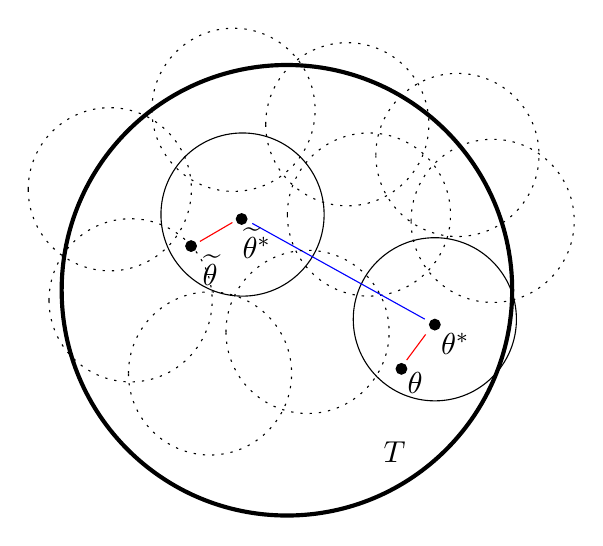
\begin{tikzpicture}[x=0.75pt,y=0.75pt,yscale=-0.87,xscale=0.87]
%uncomment if require: \path (0,365); %set diagram left start at 0, and has height of 365
%Shape: Circle [id:dp20603808590010364] 
\draw  [line width=1.5]  (194.65,169.11) .. controls (194.65,100.21) and (250.5,44.36) .. (319.4,44.36) .. controls (388.29,44.36) and (444.15,100.21) .. (444.15,169.11) .. controls (444.15,238.01) and (388.29,293.86) .. (319.4,293.86) .. controls (250.5,293.86) and (194.65,238.01) .. (194.65,169.11) -- cycle ;
%Shape: Circle [id:dp7264183031125551] 
\draw  [dash pattern={on 0.84pt off 2.51pt}] (176.14,113.18) .. controls (176.14,88.23) and (196.37,68) .. (221.32,68) .. controls (246.27,68) and (266.5,88.23) .. (266.5,113.18) .. controls (266.5,138.13) and (246.27,158.36) .. (221.32,158.36) .. controls (196.37,158.36) and (176.14,138.13) .. (176.14,113.18) -- cycle ;
%Shape: Circle [id:dp5241279298174639] 
\draw   (249.64,127.18) .. controls (249.64,102.23) and (269.87,82) .. (294.82,82) .. controls (319.77,82) and (340,102.23) .. (340,127.18) .. controls (340,152.13) and (319.77,172.36) .. (294.82,172.36) .. controls (269.87,172.36) and (249.64,152.13) .. (249.64,127.18) -- cycle ;
%Shape: Circle [id:dp7096429861126694] 
\draw  [dash pattern={on 0.84pt off 2.51pt}] (244.64,69.18) .. controls (244.64,44.23) and (264.87,24) .. (289.82,24) .. controls (314.77,24) and (335,44.23) .. (335,69.18) .. controls (335,94.13) and (314.77,114.36) .. (289.82,114.36) .. controls (264.87,114.36) and (244.64,94.13) .. (244.64,69.18) -- cycle ;
%Shape: Circle [id:dp9706226409810019] 
\draw  [dash pattern={on 0.84pt off 2.51pt}] (307.64,77.18) .. controls (307.64,52.23) and (327.87,32) .. (352.82,32) .. controls (377.77,32) and (398,52.23) .. (398,77.18) .. controls (398,102.13) and (377.77,122.36) .. (352.82,122.36) .. controls (327.87,122.36) and (307.64,102.13) .. (307.64,77.18) -- cycle ;
%Shape: Circle [id:dp6398302107173852] 
\draw  [dash pattern={on 0.84pt off 2.51pt}] (368.64,94.18) .. controls (368.64,69.23) and (388.87,49) .. (413.82,49) .. controls (438.77,49) and (459,69.23) .. (459,94.18) .. controls (459,119.13) and (438.77,139.36) .. (413.82,139.36) .. controls (388.87,139.36) and (368.64,119.13) .. (368.64,94.18) -- cycle ;
%Shape: Circle [id:dp8128828121822012] 
\draw  [dash pattern={on 0.84pt off 2.51pt}] (319.64,127.18) .. controls (319.64,102.23) and (339.87,82) .. (364.82,82) .. controls (389.77,82) and (410,102.23) .. (410,127.18) .. controls (410,152.13) and (389.77,172.36) .. (364.82,172.36) .. controls (339.87,172.36) and (319.64,152.13) .. (319.64,127.18) -- cycle ;
%Shape: Circle [id:dp05369831229990596] 
\draw  [dash pattern={on 0.84pt off 2.51pt}] (388.14,130.68) .. controls (388.14,105.73) and (408.37,85.5) .. (433.32,85.5) .. controls (458.27,85.5) and (478.5,105.73) .. (478.5,130.68) .. controls (478.5,155.63) and (458.27,175.86) .. (433.32,175.86) .. controls (408.37,175.86) and (388.14,155.63) .. (388.14,130.68) -- cycle ;
%Shape: Circle [id:dp33392831914210697] 
\draw   (356.14,185.18) .. controls (356.14,160.23) and (376.37,140) .. (401.32,140) .. controls (426.27,140) and (446.5,160.23) .. (446.5,185.18) .. controls (446.5,210.13) and (426.27,230.36) .. (401.32,230.36) .. controls (376.37,230.36) and (356.14,210.13) .. (356.14,185.18) -- cycle ;
%Shape: Circle [id:dp7376700951757287] 
\draw  [fill={rgb, 255:red, 0; green, 0; blue, 0 }  ,fill opacity=1 ] (398.36,188.14) .. controls (398.36,186.5) and (399.69,185.18) .. (401.32,185.18) .. controls (402.95,185.18) and (404.28,186.5) .. (404.28,188.14) .. controls (404.28,189.77) and (402.95,191.09) .. (401.32,191.09) .. controls (399.69,191.09) and (398.36,189.77) .. (398.36,188.14) -- cycle ;
%Shape: Circle [id:dp8002681590341161] 
\draw  [fill={rgb, 255:red, 0; green, 0; blue, 0 }  ,fill opacity=1 ] (291.36,129.64) .. controls (291.36,128) and (292.69,126.68) .. (294.32,126.68) .. controls (295.95,126.68) and (297.28,128) .. (297.28,129.64) .. controls (297.28,131.27) and (295.95,132.59) .. (294.32,132.59) .. controls (292.69,132.59) and (291.36,131.27) .. (291.36,129.64) -- cycle ;
%Shape: Circle [id:dp7359208055883519] 
\draw  [fill={rgb, 255:red, 0; green, 0; blue, 0 }  ,fill opacity=1 ] (379.86,212.64) .. controls (379.86,211) and (381.19,209.68) .. (382.82,209.68) .. controls (384.45,209.68) and (385.78,211) .. (385.78,212.64) .. controls (385.78,214.27) and (384.45,215.59) .. (382.82,215.59) .. controls (381.19,215.59) and (379.86,214.27) .. (379.86,212.64) -- cycle ;
%Shape: Circle [id:dp5092748427719243] 
\draw  [fill={rgb, 255:red, 0; green, 0; blue, 0 }  ,fill opacity=1 ] (263.36,144.64) .. controls (263.36,143) and (264.69,141.68) .. (266.32,141.68) .. controls (267.95,141.68) and (269.28,143) .. (269.28,144.64) .. controls (269.28,146.27) and (267.95,147.59) .. (266.32,147.59) .. controls (264.69,147.59) and (263.36,146.27) .. (263.36,144.64) -- cycle ;
%Straight Lines [id:da10457798813301644] 
\draw [color={rgb, 255:red, 255; green, 0; blue, 0 }  ,draw opacity=1 ]   (289.22,131.58) -- (271.22,142.08) ;
%Straight Lines [id:da7764640295404648] 
\draw [color={rgb, 255:red, 0; green, 0; blue, 255 }  ,draw opacity=1 ]   (300.22,132.08) -- (395.72,185.08) ;
%Shape: Circle [id:dp4176329073234546] 
\draw  [dash pattern={on 0.84pt off 2.51pt}] (187.64,174.68) .. controls (187.64,149.73) and (207.87,129.5) .. (232.82,129.5) .. controls (257.77,129.5) and (278,149.73) .. (278,174.68) .. controls (278,199.63) and (257.77,219.86) .. (232.82,219.86) .. controls (207.87,219.86) and (187.64,199.63) .. (187.64,174.68) -- cycle ;
%Shape: Circle [id:dp01245100707397695] 
\draw  [dash pattern={on 0.84pt off 2.51pt}] (285.64,192.18) .. controls (285.64,167.23) and (305.87,147) .. (330.82,147) .. controls (355.77,147) and (376,167.23) .. (376,192.18) .. controls (376,217.13) and (355.77,237.36) .. (330.82,237.36) .. controls (305.87,237.36) and (285.64,217.13) .. (285.64,192.18) -- cycle ;
%Straight Lines [id:da9095478885610673] 
\draw [color={rgb, 255:red, 255; green, 0; blue, 0 }  ,draw opacity=1 ]   (396.22,193.58) -- (385.72,207.75) ;
%Shape: Circle [id:dp5374996882496619] 
\draw  [dash pattern={on 0.84pt off 2.51pt}] (231.64,215.18) .. controls (231.64,190.23) and (251.87,170) .. (276.82,170) .. controls (301.77,170) and (322,190.23) .. (322,215.18) .. controls (322,240.13) and (301.77,260.36) .. (276.82,260.36) .. controls (251.87,260.36) and (231.64,240.13) .. (231.64,215.18) -- cycle ;

% Text Node
\draw (403.32,191.54) node [anchor=north west][inner sep=0.75pt]    {\large$\theta ^{*}$};
% Text Node
\draw (293.36,133.04) node [anchor=north west][inner sep=0.75pt]    {\large$\widetilde{\theta }^{*}$};
% Text Node
\draw (384.82,213.08) node [anchor=north west][inner sep=0.75pt]    {\large$\theta $};
% Text Node
\draw (271.28,148.04) node [anchor=north west][inner sep=0.75pt]    {\large$\widetilde{\theta }$};
% Text Node
\draw (371.5,251.4) node [anchor=north west][inner sep=0.75pt]    {\large$T$};
\end{tikzpicture}
\end{center}
Then, take the expectation on both sides. We use the sub-Gaussian maxima (Thm.~\ref{thm:sub-gaussian-maxima}) on $|X_{\theta_i} - X_{\theta_j}|$, which has  parameter at most $\rho(\theta_i, \theta_j) \leq \sigma$.
Therefore,
\begin{align*}
    \mathbb{E} \sup_{\theta, \theta' \in \mathbb{T}} X_\theta - X_{\theta'} \leq 2 \mathbb{E} \sup_{\theta, \theta' \in \mathbb{T}\atop \rho(\theta, \theta')\leq \delta} (X_\theta - X_{\theta'}) + 4 \sigma \sqrt{\log N(\delta)}
\end{align*}
\end{proof}
\begin{theorem}[One-step discretization bound - corollary] Let $X_\theta = \frac{1}{n} \sum_{i=1}^n \epsilon_i \theta_i$, where $\epsilon$ are Rademacher RVs. Then $\{X_\theta, \theta \in \mathbb{T} \}$ is a sub-Gaussian process with $\rho(\theta, \theta') = \frac{\norm{\theta - \theta'}_2}{\sqrt{n}}$. We have an upper bound as
\begin{align*}
    \mathcal{R}_n(T) \leq \frac{1}{\sqrt{n}} \mathbb{E} \sup_{\theta, \theta' \in \mathbb{T}} X_\theta - X_{\theta'} \leq \frac{2}{\sqrt{n}}[\delta \sqrt{n} + 2\sigma \sqrt{\log N(\delta}],
\end{align*}
\end{theorem}
\textbf{Remark}: This provides a usage of sub-Gaussian process, to bound the Rademacher complexity.

\begin{theorem}[Dudley's integral] 
Let $\{X_\theta, \theta \in \mathbb{T} \}$ be a zero-mean sub-Gaussian process with a  metric $\rho$. Define $D = \sup_{\theta, \theta'} \rho(\theta, \theta')$.
\begin{align*}
    \mathbb{E} \sup_{\theta, \theta'} X_\theta - X_{\theta'} \leq 2 \mathbb{E} \sup_{\rho(\theta, \theta')} X_\theta - X_{\theta'} + 16 \int^D_{\delta/4} \sqrt{\log N(t)} \mathrm{d}t.
\end{align*}
\end{theorem}
\textbf{Remark}: The Dudley's integral (sometimes) achieves a tighter bound on the last term of $4\sigma \sqrt{\log N(\delta)}$ by chaining method.

\begin{center}
\tikzset{every picture/.style={line width=0.75pt}} %set default line width to 0.75pt        

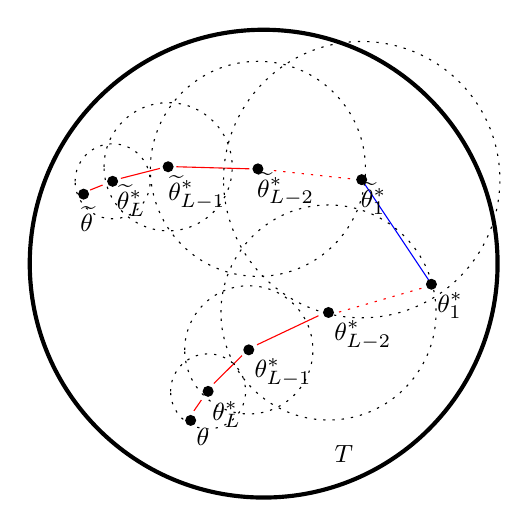
\begin{tikzpicture}[x=0.75pt,y=0.75pt,yscale=-0.8,xscale=0.8]
%uncomment if require: \path (0,365); %set diagram left start at 0, and has height of 365

%Shape: Circle [id:dp19684007366944822] 
\draw  [line width=1.5]  (221.91,172.73) .. controls (221.91,94.93) and (284.98,31.86) .. (362.78,31.86) .. controls (440.58,31.86) and (503.65,94.93) .. (503.65,172.73) .. controls (503.65,250.52) and (440.58,313.59) .. (362.78,313.59) .. controls (284.98,313.59) and (221.91,250.52) .. (221.91,172.73) -- cycle ;
%Shape: Circle [id:dp37546481991304903] 
\draw  [fill={rgb, 255:red, 0; green, 0; blue, 0 }  ,fill opacity=1 ] (326.36,249.64) .. controls (326.36,248) and (327.69,246.68) .. (329.32,246.68) .. controls (330.95,246.68) and (332.28,248) .. (332.28,249.64) .. controls (332.28,251.27) and (330.95,252.59) .. (329.32,252.59) .. controls (327.69,252.59) and (326.36,251.27) .. (326.36,249.64) -- cycle ;
%Shape: Circle [id:dp2963294714242435] 
\draw  [fill={rgb, 255:red, 0; green, 0; blue, 0 }  ,fill opacity=1 ] (268.86,123.14) .. controls (268.86,121.5) and (270.19,120.18) .. (271.82,120.18) .. controls (273.45,120.18) and (274.78,121.5) .. (274.78,123.14) .. controls (274.78,124.77) and (273.45,126.09) .. (271.82,126.09) .. controls (270.19,126.09) and (268.86,124.77) .. (268.86,123.14) -- cycle ;
%Shape: Circle [id:dp5420621191274886] 
\draw  [fill={rgb, 255:red, 0; green, 0; blue, 0 }  ,fill opacity=1 ] (315.86,267.14) .. controls (315.86,265.5) and (317.19,264.18) .. (318.82,264.18) .. controls (320.45,264.18) and (321.78,265.5) .. (321.78,267.14) .. controls (321.78,268.77) and (320.45,270.09) .. (318.82,270.09) .. controls (317.19,270.09) and (315.86,268.77) .. (315.86,267.14) -- cycle ;
%Shape: Circle [id:dp9995668227699503] 
\draw  [fill={rgb, 255:red, 0; green, 0; blue, 0 }  ,fill opacity=1 ] (251.37,130.87) .. controls (251.37,129.24) and (252.69,127.91) .. (254.32,127.91) .. controls (255.96,127.91) and (257.28,129.24) .. (257.28,130.87) .. controls (257.28,132.5) and (255.96,133.83) .. (254.32,133.83) .. controls (252.69,133.83) and (251.37,132.5) .. (251.37,130.87) -- cycle ;
%Straight Lines [id:da6606938671394016] 
\draw [color={rgb, 255:red, 255; green, 0; blue, 0 }  ,draw opacity=1 ]   (265.78,125.37) -- (258.28,128.37) ;
%Straight Lines [id:da31124628774224106] 
\draw [color={rgb, 255:red, 0; green, 0; blue, 255 }  ,draw opacity=1 ]   (421.82,122.14) -- (463.82,185.14) ;
%Shape: Circle [id:dp6240904030753718] 
\draw  [dash pattern={on 0.84pt off 2.51pt}] (306.73,249.64) .. controls (306.73,237.16) and (316.85,227.05) .. (329.32,227.05) .. controls (341.8,227.05) and (351.91,237.16) .. (351.91,249.64) .. controls (351.91,262.11) and (341.8,272.22) .. (329.32,272.22) .. controls (316.85,272.22) and (306.73,262.11) .. (306.73,249.64) -- cycle ;
%Straight Lines [id:da02663647664030422] 
\draw [color={rgb, 255:red, 255; green, 0; blue, 0 }  ,draw opacity=1 ]   (325.28,254.87) -- (320.78,261.37) ;
%Shape: Circle [id:dp0641440846668293] 
\draw  [fill={rgb, 255:red, 0; green, 0; blue, 0 }  ,fill opacity=1 ] (302.28,114.37) .. controls (302.28,112.74) and (303.6,111.41) .. (305.24,111.41) .. controls (306.87,111.41) and (308.19,112.74) .. (308.19,114.37) .. controls (308.19,116) and (306.87,117.33) .. (305.24,117.33) .. controls (303.6,117.33) and (302.28,116) .. (302.28,114.37) -- cycle ;
%Straight Lines [id:da6203583479569572] 
\draw [color={rgb, 255:red, 255; green, 0; blue, 0 }  ,draw opacity=1 ]   (300.28,115.37) -- (276.78,121.37) ;
%Shape: Circle [id:dp35910966149356827] 
\draw  [fill={rgb, 255:red, 0; green, 0; blue, 0 }  ,fill opacity=1 ] (356.36,115.64) .. controls (356.36,114) and (357.69,112.68) .. (359.32,112.68) .. controls (360.95,112.68) and (362.28,114) .. (362.28,115.64) .. controls (362.28,117.27) and (360.95,118.59) .. (359.32,118.59) .. controls (357.69,118.59) and (356.36,117.27) .. (356.36,115.64) -- cycle ;
%Straight Lines [id:da2672880550331598] 
\draw [color={rgb, 255:red, 255; green, 0; blue, 0 }  ,draw opacity=1 ]   (354.19,115.61) -- (310.19,114.37) ;
%Shape: Circle [id:dp3275093497755006] 
\draw  [fill={rgb, 255:red, 0; green, 0; blue, 0 }  ,fill opacity=1 ] (350.86,224.64) .. controls (350.86,223) and (352.19,221.68) .. (353.82,221.68) .. controls (355.45,221.68) and (356.78,223) .. (356.78,224.64) .. controls (356.78,226.27) and (355.45,227.59) .. (353.82,227.59) .. controls (352.19,227.59) and (350.86,226.27) .. (350.86,224.64) -- cycle ;
%Straight Lines [id:da06735315583419843] 
\draw [color={rgb, 255:red, 255; green, 0; blue, 0 }  ,draw opacity=1 ]   (349.78,228.09) -- (332.78,244.87) ;
%Shape: Circle [id:dp962698819630809] 
\draw  [fill={rgb, 255:red, 0; green, 0; blue, 0 }  ,fill opacity=1 ] (398.86,202.14) .. controls (398.86,200.5) and (400.19,199.18) .. (401.82,199.18) .. controls (403.45,199.18) and (404.78,200.5) .. (404.78,202.14) .. controls (404.78,203.77) and (403.45,205.09) .. (401.82,205.09) .. controls (400.19,205.09) and (398.86,203.77) .. (398.86,202.14) -- cycle ;
%Straight Lines [id:da8264622210983994] 
\draw [color={rgb, 255:red, 255; green, 0; blue, 0 }  ,draw opacity=1 ]   (395.78,204.09) -- (358.78,221.59) ;
%Shape: Circle [id:dp12588135320242566] 
\draw  [fill={rgb, 255:red, 0; green, 0; blue, 0 }  ,fill opacity=1 ] (460.86,185.14) .. controls (460.86,183.5) and (462.19,182.18) .. (463.82,182.18) .. controls (465.45,182.18) and (466.78,183.5) .. (466.78,185.14) .. controls (466.78,186.77) and (465.45,188.09) .. (463.82,188.09) .. controls (462.19,188.09) and (460.86,186.77) .. (460.86,185.14) -- cycle ;
%Shape: Circle [id:dp79173620737152] 
\draw  [fill={rgb, 255:red, 0; green, 0; blue, 0 }  ,fill opacity=1 ] (418.86,122.14) .. controls (418.86,120.5) and (420.19,119.18) .. (421.82,119.18) .. controls (423.45,119.18) and (424.78,120.5) .. (424.78,122.14) .. controls (424.78,123.77) and (423.45,125.09) .. (421.82,125.09) .. controls (420.19,125.09) and (418.86,123.77) .. (418.86,122.14) -- cycle ;
%Straight Lines [id:da1378960949499275] 
\draw [color={rgb, 255:red, 255; green, 0; blue, 0 }  ,draw opacity=1 ] [dash pattern={on 0.84pt off 2.51pt}]  (414.78,121.59) -- (366.19,116.37) ;
%Straight Lines [id:da5506540246280685] 
\draw [color={rgb, 255:red, 255; green, 0; blue, 0 }  ,draw opacity=1 ] [dash pattern={on 0.84pt off 2.51pt}]  (457.78,187.59) -- (408.19,201.87) ;
%Shape: Circle [id:dp2677220432717424] 
\draw  [dash pattern={on 0.84pt off 2.51pt}] (315.22,224.64) .. controls (315.22,203.32) and (332.5,186.04) .. (353.82,186.04) .. controls (375.14,186.04) and (392.42,203.32) .. (392.42,224.64) .. controls (392.42,245.95) and (375.14,263.24) .. (353.82,263.24) .. controls (332.5,263.24) and (315.22,245.95) .. (315.22,224.64) -- cycle ;
%Shape: Circle [id:dp20125267536050773] 
\draw  [dash pattern={on 0.84pt off 2.51pt}] (337.04,202.14) .. controls (337.04,166.36) and (366.04,137.36) .. (401.82,137.36) .. controls (437.6,137.36) and (466.6,166.36) .. (466.6,202.14) .. controls (466.6,237.91) and (437.6,266.91) .. (401.82,266.91) .. controls (366.04,266.91) and (337.04,237.91) .. (337.04,202.14) -- cycle ;
%Shape: Circle [id:dp29151738350801537] 
\draw  [dash pattern={on 0.84pt off 2.51pt}] (249.23,123.14) .. controls (249.23,110.66) and (259.35,100.55) .. (271.82,100.55) .. controls (284.3,100.55) and (294.41,110.66) .. (294.41,123.14) .. controls (294.41,135.61) and (284.3,145.72) .. (271.82,145.72) .. controls (259.35,145.72) and (249.23,135.61) .. (249.23,123.14) -- cycle ;
%Shape: Circle [id:dp9553417291902377] 
\draw  [dash pattern={on 0.84pt off 2.51pt}] (266.64,114.37) .. controls (266.64,93.05) and (283.92,75.77) .. (305.24,75.77) .. controls (326.55,75.77) and (343.84,93.05) .. (343.84,114.37) .. controls (343.84,135.69) and (326.55,152.97) .. (305.24,152.97) .. controls (283.92,152.97) and (266.64,135.69) .. (266.64,114.37) -- cycle ;
%Shape: Circle [id:dp1802524110332464] 
\draw  [dash pattern={on 0.84pt off 2.51pt}] (294.54,115.64) .. controls (294.54,79.86) and (323.54,50.86) .. (359.32,50.86) .. controls (395.1,50.86) and (424.1,79.86) .. (424.1,115.64) .. controls (424.1,151.41) and (395.1,180.41) .. (359.32,180.41) .. controls (323.54,180.41) and (294.54,151.41) .. (294.54,115.64) -- cycle ;
%Shape: Circle [id:dp03052433859047765] 
\draw  [dash pattern={on 0.84pt off 2.51pt}] (338.62,122.14) .. controls (338.62,76.18) and (375.87,38.93) .. (421.82,38.93) .. controls (467.77,38.93) and (505.03,76.18) .. (505.03,122.14) .. controls (505.03,168.09) and (467.77,205.34) .. (421.82,205.34) .. controls (375.87,205.34) and (338.62,168.09) .. (338.62,122.14) -- cycle ;

% Text Node
\draw (330.32,254.04) node [anchor=north west][inner sep=0.75pt]    {$\theta _{L}^{*}$};
% Text Node
\draw (272.82,123.58) node [anchor=north west][inner sep=0.75pt]    {$\widetilde{\theta }_{L}^{*}$};
% Text Node
\draw (320.82,270.54) node [anchor=north west][inner sep=0.75pt]    {$\theta $};
% Text Node
\draw (250.78,136.54) node [anchor=north west][inner sep=0.75pt]    {$\widetilde{\theta }$};
% Text Node
\draw (404,280.4) node [anchor=north west][inner sep=0.75pt]    {$T$};
% Text Node
\draw (303.82,118.04) node [anchor=north west][inner sep=0.75pt]    {$\widetilde{\theta }_{L-1}^{*}$};
% Text Node
\draw (357.32,116.04) node [anchor=north west][inner sep=0.75pt]    {$\widetilde{\theta }_{L-2}^{*}$};
% Text Node
\draw (355.82,228.04) node [anchor=north west][inner sep=0.75pt]    {$\theta _{L-1}^{*}$};
% Text Node
\draw (403.82,205.54) node [anchor=north west][inner sep=0.75pt]    {$\theta _{L-2}^{*}$};
% Text Node
\draw (465.82,188.54) node [anchor=north west][inner sep=0.75pt]    {$\theta _{1}^{*}$};
% Text Node
\draw (419.82,122.54) node [anchor=north west][inner sep=0.75pt]    {$\widetilde{\theta }_{1}^{*}$};


\end{tikzpicture}
\end{center}
\begin{proof}
Define $L = \ceil{\log_2 \frac{D}{\delta} }$ sets of $\delta_i$-covers $\mathcal{C}_i$, where $\delta_i = \frac{1}{2^i}D$. Let $N(\delta_i)$ denote the covering number in $\mathcal{C}_i$.
\begin{align*}
X_{\theta_{L}}-X_{\widetilde{\theta_{L}}} & \leq {\color{red} X_{\theta_L}-X_{\theta^*_{L-1}}} + {\color{blue} X_{\theta^*_{L-1}}-X_{\widetilde{\theta}^*_{L-1}}}+{\color{red}X_{\widetilde{\theta}^{\star}_{L-1}}-X_{\widetilde{\theta_L}}} \\
&= {\color{red} 2 \max _{\theta \in \mathcal{C}_{L}} X_{\theta}-X_{\theta^*_{L-1}}} + {\color{blue}\max_{\theta, \theta^{\prime} \in \mathcal{C}_{L-1}} X_{\theta}-X_{\theta^{\prime}}} \\
& \cdots\cdots \\
& \leq  {\color{red}2 \sum_{i=2}^{L} \max_{\theta \in \mathcal{C}_{i}} X_{\theta}-X_{\theta^*_{i-1}}} + {\color{blue}\max _{\theta, \theta^{\prime} \in \mathcal{C}_{1}} X_{\theta}-X_{\theta^{\prime}}}
\end{align*}
Next, we use sub-Gaussian maxima,
\begin{align*}
    \EE \, {\color{red}\max_{\theta \in \mathcal{C}_{i}} X_{\theta}-X_{\theta^*_{i-1}}} & \leq 2 \delta_{i-1} \sqrt{\log |\mathcal{C}_i|} \leq 2 \cdot \frac{D}{2^{i-1}} \sqrt{\log N\left(\frac{D}{2^{i-1}}\right)} \\
    & \leq 8 \int_{D/2^{i-1}}^{D/2^i} \sqrt{\log N\left(t\right)} \mathrm{d} t
\end{align*}
Putting things together, we get
\begin{align*}
\mathbb{E} \max _{\theta, \tilde{\theta} \in \mathcal{C}_{L}} X_{\theta}-X_{\tilde{\theta}} & \leq 16 \sum_{i=2}^{L}\int_{\frac{D}{2^{i-1}}}^{\frac{D}{2^i}} \sqrt{\log N\left(t\right)} \mathrm{d} t + 2 D \sqrt{\log N\left(\frac{D}{2}\right)} \\
& \leq 16 \int_{\delta / 4}^{D} \sqrt{\log N_{\mathbb{T}}(t)} \mathrm{d} t
\end{align*}
This gives the desired form.
\end{proof}



\section{Reproducing Kernel Hilbert Spaces (Ch. 12)}
\subsection{Basics of Hilbert space}

\begin{definition}[Hilbert spaces]
A Hilbert space $\mathcal{H}$ is a complete inner product space. In a Hilbert space
\begin{itemize}
    \item There endows an inner product: $\langle \cdot, \cdot, \rangle_\mathcal{H}$,
    \item Every Cauchy sequence $(f_n)_{n=1}^\infty$ in $\mathcal{H}$ converges to some element $f^* \in \mathcal{H}$.
\end{itemize}
\end{definition}

\begin{theorem}[Riesz representation]
Let $L$ be a bounded linear functional on a Hilbert space $\mathcal{H}$. Then there exists a unique representer $g\in \mathcal{H}$ such that $L(f) = \langle f, g \rangle_\mathcal{H}$ for all $f \in H$.
\end{theorem}
\begin{proof}
Consider a null space $\mathrm{Null}(L) := \{h \mid L(h) = 0\}$. If $\mathrm{Null}(L) = H$, then $\mathrm{Null}(L)^\bot = \{0\}$, we take $g = 0$. 

In a non-trivial case (i.e., $\mathrm{Null}(L)^\bot \neq \{0\}$), there exist a non-zero element $g \in \mathrm{Null}(L)^\bot$ such that $\norm{g}_\mathcal{H} = L(g)$. Define $h:= L(f) g - L(g) f$, then we note
\begin{align*}
    L(h) = L(f) L(g) - L(g) L(f) = 0,
\end{align*}
which means $h \in \mathrm{Null}(L)$. Therefore, we have $h \bot g$, i.e.,
\begin{align*}
    0 & = \langle h, g \rangle_\mathcal{H} = L(f) \norm{g}^2_\mathcal{H} - L(g) \langle f, g \rangle_\mathcal{H}.
\end{align*}
This implies $L(f) = \langle f, g \rangle_\mathcal{H}$.
\end{proof}
\begin{table*}[t]
\center
        \begin{tabular}{lll}
    \toprule
         Space & Kernel & Eigenfunctin  \\
    \midrule
         $2$-poly. & $K(x, z) = (1 + xz)^2$ & $\phi_j(x) = a_0^j + a_1^j x + a_2^j x^2$, const via eigen-decomposition.  \\
         $1$-Sobolev $W_2^1([0,1])$ & $K(x, z) = \min \{x, z\}$ & $\phi_j(t)=\sin \frac{(2j-1)\pi t}{2}, \mu_j = \left(\frac{2}{(2j-1)\pi} \right)^2$ \\
    \bottomrule
    \end{tabular}
\end{table*}

\subsection{Reproducing kernel Hilbert space}
\begin{definition}[Kernel function]
Given a feature map $\phi: \mathcal{X} \rightarrow \mathcal{H}$ and the Hilbert space $\mathcal{H}$ that $\phi$ maps to, the kernel function is defined as $$ K(x, y) := \langle \phi(x), \phi(y) \rangle_\mathcal{H}.
$$
\end{definition}

\begin{definition}[RKHS - defined by kernel] A reproducing kernel Hilbert space is a Hilbert space $\mathcal{H}$ of functions $f: \mathcal{X} \rightarrow \R$  with a kernel function $K(\cdot, \cdot)$ that
\begin{itemize}
    \item For any $x \in \mathcal{X}$, $K(\cdot, x) \in \mathcal{H}$,
    \item Satisfies the ``reproducing property'':$$
    \langle f(\cdot), K(\cdot, x) \rangle_\mathcal{H} = f(x), \quad \forall f \in \mathcal{H}.
$$
\end{itemize}
\end{definition}

\begin{theorem}[RKHS from kernel function]
Given any positive semi-definite kernel function $K(\cdot, \cdot)$, there is a \textbf{unique} Hilbert space $\mathcal{H}$ in which the kernel $K(\cdot, \cdot)$ satisfies the reproducing property. 

Given some data $\{x_i\}_{i=1}^n $, such Hilbert space $\mathcal{H}$ is 
$$
\mathcal{H} := \left\{ f(\cdot) = \sum_{i=1}^n \alpha_i K(\cdot, x_i)\ \bigg|\ x_i \in \mathcal{X} \right\}$$
with the norm
$$
\langle f, f' \rangle_\mathcal{H} := \sum_{i=1}^n  \sum_{j=1}^n \alpha_i \alpha'_j K(x_i, x_j)  
$$
\end{theorem}
\textbf{Remark}: For a fixed kernel function, there will be (infinitely) many feature maps, and thus many Hilbert spaces of the feature. But the Hilbert space that \textbf{satisfies the reproducing property} is unique!

\begin{definition}[RKHS - defined by evaluation functional] A reproducing kernel Hilbert space is a Hilbert space $\mathcal{H}$ of functions $f: \mathcal{X} \rightarrow \R$ such that for each $x \in \mathcal{X}$, the evaluation functional $L_x: \mathcal{H} \rightarrow \R$ that performs the operation $L_x(f) = f(x)$ is bounded, i.e.,
$$
f(x) = |L_x(f)| \leq M \norm{f}_\mathcal{H}, \quad \exists M < \infty,  \forall f \in \mathcal{H}.
$$
\end{definition}
\begin{proof}
Let's prove the equivalence to the first definition.

When $L_x$ is a bounded linear functional, the Riesz theorem shows that there exists a unique $R_x \in \mathcal{H}$ such that
$$
L_x(f) = \langle f, R_x \rangle_\mathcal{H}.
$$
Similarly, we can get a unique $R_y$ based on $y$. The kernel is defined as $K(x, y) = \langle R_x, R_y \rangle_\mathcal{H}$. Next, we can verify that $K$ is positive semidefinite.
\begin{align*}
    \alpha^T K \alpha & = \sum_{i=1}^n \sum_{j=1}^n \alpha_i \alpha_j K(x_i, x_j) = \langle \sum_{i=1}^n \alpha_i R_{x_i}, \sum_{j=1}^n \alpha_j R_{x_j} \rangle_\mathcal{H} \\
    & = \norm{\sum_{i=1}^n \alpha_i R_{x_i}}^2_\mathcal{H} \geq 0.
\end{align*}
\end{proof}

\subsection{Mercer's theorem and its consequences}
\begin{theorem}[Mercer's]
For a continuous and PSD kernel function $K$ that satisfies the Hilbert-Schmidt condition. Then there exist a sequence of eigenfunctions $(\phi_i)_{i=1}^\infty$ that form an orthonormal basis of $L^2(\mathcal{X}; P)$ and non-negative eigenvalues $(\mu_i)_{i=1}^\infty$ such that
\begin{align}
    T_K(\phi_i) = \mu_i \phi_i, \quad \forall i=1,2,\cdots
\end{align}
Moreover, the kernel function has the expansion
\begin{align*}
    K(x, y) = \langle \Phi(x), \Phi(y) \rangle_{\ell^2(\mathbb{N)}} := \sum_{i=1}^\infty \mu_i \phi_i(x) \phi_j(y)
\end{align*}
\end{theorem}
\section{Non-parametric Least Squares (Ch. 13)}

\subsection{Fixed design}

\begin{definition}[Least square regression]
For a function $f^*$ and data collection $\{(x_i, y_i)\}_{i=1}^n$, where $y_i = f^*(x_i) + \sigma w_i$, $w_i \sim \NN{0, 1}$, the least-squares estimateor estimator is given by
$$
\hat{f} = \arg \min_{f\in\mathcal{F}} \frac{1}{n} \sum_{i=1}^{n} (y_i - f(x_i))^2.
$$
\end{definition}

\begin{property}[Basic inequality] In the non-parametric least squares, we have the optimality of $\hat{f}$, which means
$$
\frac{1}{n} \sum_{i=1}^{n}\left(\hat{f}\left(x_{i}\right)-y_{i}\right)^{2} \leq \frac{1}{n} \sum_{i=1}^{n}\left(f^{*}\left(x_{i}\right) - y_{i}\right)^{2}
$$
Or, equivalently,
$$
\left\|f-f^{*}\right\|_{n}^{2} \leq \frac{2 \sigma}{n} \sum_{i=1}^{n} w_{i}\left(f\left(x_{i}\right)-f^{*}\left(x_{i}\right)\right).
$$
\end{property}
\begin{proof}
Let's prove the equivalence. Note that $y_i = f^*(x_i) + \sigma w_i$, we have 
\begin{align*}
    0 & \geq \frac{1}{n} \sum_{i=1}^{n}\left(\hat{f}\left(x_{i}\right)-y_{i}\right)^{2} - \frac{1}{n} \sum_{i=1}^{n}\left(f^{*}\left(x_{i}\right) - y_{i}\right)^{2} \\
    & \geq \frac{1}{n} \sum_{i=1}^{n} \left( (\hat{f}(x_i)^2 - f^*(x_i)^2) - 2y_i (\hat{f}(x_i) - f^*(x_i)) \right) \\
    & \geq \frac{1}{n} \sum_{i=1}^{n} \left( (\hat{f}(x_i) - f^*(x_i))^2 - 2\sigma w_i (\hat{f}(x_i) - f^*(x_i))\right),
\end{align*}
which means
$$
\frac{1}{n} \sum_{i=1}^{n} \left( (\hat{f}(x_i) - f^*(x_i))^2 \right) \leq \frac{2 \sigma}{n} \sum_{i=1}^{n} \left( w_i (\hat{f}(x_i) - f^*(x_i)) \right).
$$
\end{proof}

\begin{definition}[Localized Gaussian complexity] If we restrict the radius of function space $\mathcal{F}$, i.e., $\norm{f}_n \leq \delta$, we have the localized Gaussian complexity for $\mathcal{F}$,
$$
{\mathcal{G}}_n\left(\delta ; \mathcal{F}\right):=\mathbb{E}_{w \sim \mathcal{N}(0,1)}\left[\sup _{f \in \mathcal{F},\|f\|_{n} \leq \delta} \frac{1}{n} \sum_{i=1}^{n} w_{i} f\left(x_{i}\right)\right]
$$
\end{definition}

\begin{definition}[Critical radius]
For a local Gaussian complexity $\mathcal{G}_{n}$ around $f^*$ with radius $\delta$, the radius $\delta$ is said to be \textit{valid} if the following \textit{critical inequality} satisfies,
$$
\frac{\mathcal{G}_{n}\left(\delta ; \mathcal{F}^{*}\right)}{\delta} \leq \frac{\delta}{2 \sigma}
$$
The smallest $\delta$ satisfies it is the \textit{critical radius}, which must exist for any star-shaped function class $\mathcal{F}$.
\end{definition}

\textbf{Remark}: One intuition is that the satisfaction of critical inequality means the optimality of $\hat{f}$. One example is that if we have the optimality of $\hat{f}$, i.e.,
\begin{align*}
    \frac{1}{2 n} \sum_{i=1}^{n}\left(y_{i}-\widehat{f}\left(x_{i}\right)\right)^{2} \leq \frac{1}{2 n} \sum_{i=1}^{n}\left(y_{i}-f^{*}\left(x_{i}\right)\right)^{2}
\end{align*}
And let $\delta = \EE \norm{\hat{f} - f^*}_n$, then we can show the $\delta$ satisfies $\frac{1}{2} \delta^{2} \leq \sigma \mathcal{G}_{n}\left(\delta ; \mathcal{F}^{*}\right)$, which is equivalent to the critical inequality.


\begin{theorem}[Risk decomposition] In the least-squares regression, where $y_i = f^*(x_i) + \sigma w_i, w_i \sim \NN(0,1)$, we have risk decomposition
$$
R(f)=\left(\EE f(x) - \EE f^*(x)\right)^2 + \mathrm{var}\left(f(x)\right) + \sigma^{2}
$$
\end{theorem}
\begin{proof} Using the fact $ \mathrm{var}(x) =  \EE x^2 - (\EE x)^2 $ and the independence of $y$ and $f(x)$, we have
\begin{align*}
    R(f) & = \EE\left[(y - f(x))^2\right] \\
         & = \EE y^2 + \EE f(x)^2 - 2 \EE y f(x) \qquad (y \text{ and } f(x) \text{ are indep.})\\
         & = \mathrm{var}\left(y\right) + \left(\EE y\right)^2 + \mathrm{var}\left((f(x)\right) - \left(\EE f(x)\right)^2 + 2 (\EE y) (\EE f(x)) \\
         & = \mathrm{var}\left(y\right) + \mathrm{var}\left(f(x)\right)  + \left(\EE f(x) - \EE y\right)^2 \\
         & =\underbrace{\left(\EE f(x) - \EE f^*(x)\right)^2}_{\text{bias}^2} + \underbrace{\mathrm{var}\left(f(x)\right)}_{\text{variance}} + \underbrace{\sigma^2}_{\text{irreducible noise}}.
\end{align*}
If there is no variance in model, we can also get the decomposition  as,
\begin{align*}
R(f) &= \mathbb{E} \frac{1}{n} \sum_{i=1}^{n}\left(y_i -f\left(x_{i}\right)\right)^{2} \\
&= \mathbb{E} \frac{1}{n} \sum_{i=1}^{n}\left(f^{*}\left(x_{i}\right)+ \sigma w_i -f\left(x_{i}\right)\right)^{2} \\
&=\mathbb{E} \frac{1}{n} \sum_{i=1}^{n}\left(f^{*}\left(x_{i}\right)-f\left(x_{i}\right)\right)^{2}+ \mathbb{E} \frac{1}{n} \sum_{i=1}^{n} \sigma^2 w^{2} \\ 
& \quad +2 \mathbb{E} \frac{1}{n} \sum_{i=1}^{n}  w\left(f^{*}\left(x_{i}\right)-f\left(x_{i}\right)\right) \\
& = \left\|f-f^{*}\right\|_{n}^{2}+\sigma^{2}
\end{align*}
\end{proof}
\begin{theorem}[Prediction error bound]
If $\mathcal{F}^*$ is star-shaped, then for any $\delta$ satisfies the critical inequality and $t \geq \delta$, the non-parametric least square estimate $\hat{f}_n$ satisfies
$$P\left(\norm{\hat{f}_n -f^{*}}_{n}^{2} \geq 16 t \delta_{n}\right) \leq \exp \left(-\frac{n t \delta_{n}}{2 \sigma^{2}}\right),$$
which also means for some constant $c$,
$$
\EE \norm{\hat{f}_n -f^{*}}_{n}^{2} \leq c \left( \delta_n^2 + \frac{\sigma^2}{n} \right).
$$
\end{theorem}
\textbf{Remark}: This theorem links the local Gaussian complexity to the error bounds.

\begin{proof}
Let $\hat{\Delta} = f - f^*$, and thus $\norm{\hat{\Delta}} = \norm{f - f^*}_n^2$. Our goal is to show for any $\norm{\hat{\Delta}}_n \geq \sqrt{t} \delta_n$,
\begin{align*}
    \|\hat{\Delta}\|_{n}^{2} \leq \frac{2 \sigma}{n} \sum_{i=1}^{n} w_{i} \hat{\Delta}\left(x_{i}\right) \stackrel{(i)} \leq 4\|\hat{\Delta}\|_{n} \sqrt{t} \delta_{n}
\end{align*}
with probability $1 - e^{- \frac{n t \delta^2_n}{2 \sigma^2}}$. The theorem follows from rearranging terms.
We organize the proof in multiple steps.

For a given scalar $u \geq \delta_n$, define the event
$$
\mathcal{A}(u):=\left\{\exists g \in \mathcal{F}^{*} \cap \{\norm{g}_{n} \geq u\}\, \bigg| \, \left| \frac{\sigma}{n} \sum_{i=1}^{n} \tilde{w}_{i} g\left(x_{i}\right) \right| \geq 2u\norm{g}_{n}\right\}
$$
\end{proof}

\begin{theorem}[Bounds via metric entropy]
Any $\delta \in (0, \sigma]$ such that
\begin{align*}
    \frac{16}{\sqrt{n}} \int_{\frac{\delta^{2}}{4 \sigma}}^{\delta} \sqrt{\log N_{n}\left(t ; \mathbb{B}_{n}\left(\delta ; \mathscr{F}^{*}\right)\right)} d t \leq \frac{\delta^{2}}{4 \sigma}
\end{align*}
satisfies the critical inequality. 
\end{theorem}

\subsection{Error bounds for RKHS}

\begin{definition}[$R$-restrained space] The function space inside the radius $R$ is
$$
\mathcal{F}_{R}:=\left\{f \in \mathcal{F} \mid\|f\|_{\mathcal{F}} \leq R\right\}
$$
\end{definition}
\begin{theorem}[Localized Gaussian complexity for RKHS]
Let an RKHS $\mathcal{F}$ with kernel function $K(\cdot, \cdot)$. Defining $\hat{\mu}_j$ as eigenvalues of the kernel matrix $K$, we have the local Gaussian complexity bounded by
$$
{\mathcal{G}}_{n}\left(\delta; \mathcal{F}_{R}\right) \leq \sqrt{\frac{R + 1}{n}} \sqrt{\sum_{j=1}^{n} \min \left\{\delta^{2}, \hat{\mu}_{j}\right\}}
$$
Note that the localized Gaussian complexity is computed under  $\norm{f}_\mathcal{F} \leq R, \norm{f}_n \leq \delta$.
\end{theorem}

\begin{theorem}[Prediction error for norm-bounded RKHS]
When $\lambda_n \geq 2 \delta^2_{n;R}$ there is universal constants $c_0, c_1, c_3$ such that
$$
P\left(\left\|\widehat{f}_{\lambda_{n}}-f^{\star}\right\|_{n}^{2} \geq c R^{2}\left(\delta_{n ; R}^{2}+\lambda_{n}\right) \right) \leq c_{0} e^{-c_{1} \frac{n R^{2} \delta_{n: R}^{2}}{\sigma^{2}}}
$$
\end{theorem}

\subsection{Random design}
\textit{WIP...}
\end{multicols}

\end{document}
